\documentclass[
	12pt, % Font size
	a4paper, % Paper size
	twoside, % Two-sided
]{report}

% Set the PDF version for LuaTeX
\usepackage{luacode}
\begin{luacode}
  pdf.setminorversion(6)
\end{luacode}

% Packages
\usepackage[english]{babel} % Set document language
\usepackage{pdfpages} % Include PDF files
\usepackage[utf8]{inputenc} % UTF-8 encoding (for umlauts etc.)
\usepackage[T1]{fontenc} % correct hyphenation
\usepackage{csquotes} % correct quotation marks
\usepackage{lmodern} % Computer Modern fonts
\usepackage{microtype} % better typesetting results (avoids underfull / overfull hboxes)
\usepackage{graphicx} % adding graphics
\usepackage{units} % typesetting units, e.g. \unit[10]{MB} and \unitfrac[100]{Mbit}{s}
\usepackage{booktabs} % publication quality tables
\usepackage{titlesec} % Customize chapter and section headings
\usepackage{setspace} % Set line spacing
\usepackage{geometry} % Set page margins
\usepackage{subcaption} % Subfigures
\usepackage{float} % Floats
\usepackage[
	backend=bibtex,
	style=numeric-comp,
	maxcitenames=2,
	natbib=true,
	sorting=none
]{biblatex} % Bibliography
\usepackage{hyperref} % Hyperlinks
\usepackage[super]{nth} % Superscript for numbers
\usepackage{amsmath} % Math symbols
\usepackage{amssymb} % Math symbols
\usepackage{mathtools} % Math symbols
\usepackage{amsthm} % Math symbols
\usepackage[
	ruled,
	linesnumbered,
	algochapter
]{algorithm2e} % Algorithms
\usepackage{bm} % Bold math symbols
\usepackage{tikz} % Drawing

% Bibliography
\addbibresource{literature.bib}

% Custom Definitions
% Theorems %
\newtheorem{theorem}{Theorem}
\numberwithin{theorem}{chapter}
\newtheorem{definition}{Definition}
\numberwithin{definition}{chapter}
\newtheorem{corollary}{Corollary}
\numberwithin{corollary}{chapter}
\theoremstyle{remark}
\newtheorem{note}{Note}
\numberwithin{note}{chapter}

% Algorithm2e Keywords %
\SetKwBlock{Loop}{loop}{}
\SetKw{Break}{break}
\SetKw{None}{None}

% Functions &
\newcommand{\polyhedron}[1]{\mathcal{#1}}
\newcommand{\mat}[1]{{\bm{#1}}}
\renewcommand{\vec}[1]{{\bm{#1}}}
\newcommand{\conv}[0]{\operatorname{conv}}
\newcommand{\raycone}[0]{\operatorname{cone}}
\newcommand{\transpose}[0]{^\intercal}
\renewcommand{\setminus}{\backslash}
\newcommand{\rank}[0]{\operatorname{rank}}
\newcommand{\st}[0]{\operatorname{s.t.}}
\newcommand{\LP}[0]{\textit{LP}}
\newcommand{\IP}[0]{\textit{IP}}
\newcommand{\MP}[0]{\textit{MP}}
\newcommand{\RMP}[0]{\textit{RMP}}
\newcommand{\SP}[1]{{\textit{SP}\ifstrempty{#1}{}{^{#1}}}}
\newcommand{\RCP}[0]{\textit{RCP-SP}}
\newcommand{\FP}[0]{\textit{FP-SP}}
\newcommand{\indexset}[1]{\mathcal{#1}}

% Math %

\DeclarePairedDelimiter\abs{\lvert}{\rvert}%
\DeclarePairedDelimiter\norm{\lVert}{\rVert}%
\DeclarePairedDelimiter\floor{\lfloor}{\rfloor}
\DeclarePairedDelimiter\ceil{\lceil}{\rceil}

% Swap the definition of \abs* and \norm*, so that \abs
% and \norm resizes the size of the brackets, and the
% starred version does not.
\makeatletter
\let\oldabs\abs
\def\abs{\@ifstar{\oldabs}{\oldabs*}}
%
\let\oldnorm\norm
\def\norm{\@ifstar{\oldnorm}{\oldnorm*}}
\makeatother

\let\oldbar\bar
\newcommand{\ubar}[1]{{\underaccent{\oldbar}{#1}}}
\renewcommand{\bar}[1]{{\oldbar{#1}}}


% Document
\begin{document}

\begin{titlepage}
	\centering
	{\Huge\bfseries Component Bound Branching in a Branch-and-Price Framework\par}
	\vspace{0.85cm}
	{\LARGE Master Thesis in Computer Science\\RWTH Aachen University\par}
	\vspace{2cm}
	{\LARGE Til Mohr\par}
	\vspace{0.5cm}
	{\large til.mohr@rwth-aachen.de\\Student ID: 405959\par}
	\vspace{2cm}
	{\large \today\par}
	\vspace{2cm}
	\begin{minipage}{0.48\textwidth}
		\centering
		\nth{1} Examiner\\
		Prof. Dr. Peter Rossmanith\\
		Chair of Theoretical Computer Science\\
		RWTH Aachen University
	\end{minipage}
	\begin{minipage}{0.48\textwidth}
		\centering
		\nth{2} Examiner\\
		Prof. Dr. Marco Lübbecke\\
		Chair of Operations Research\\
		RWTH Aachen University
	\end{minipage}
\end{titlepage}

% Eidesstattliche Versicherung
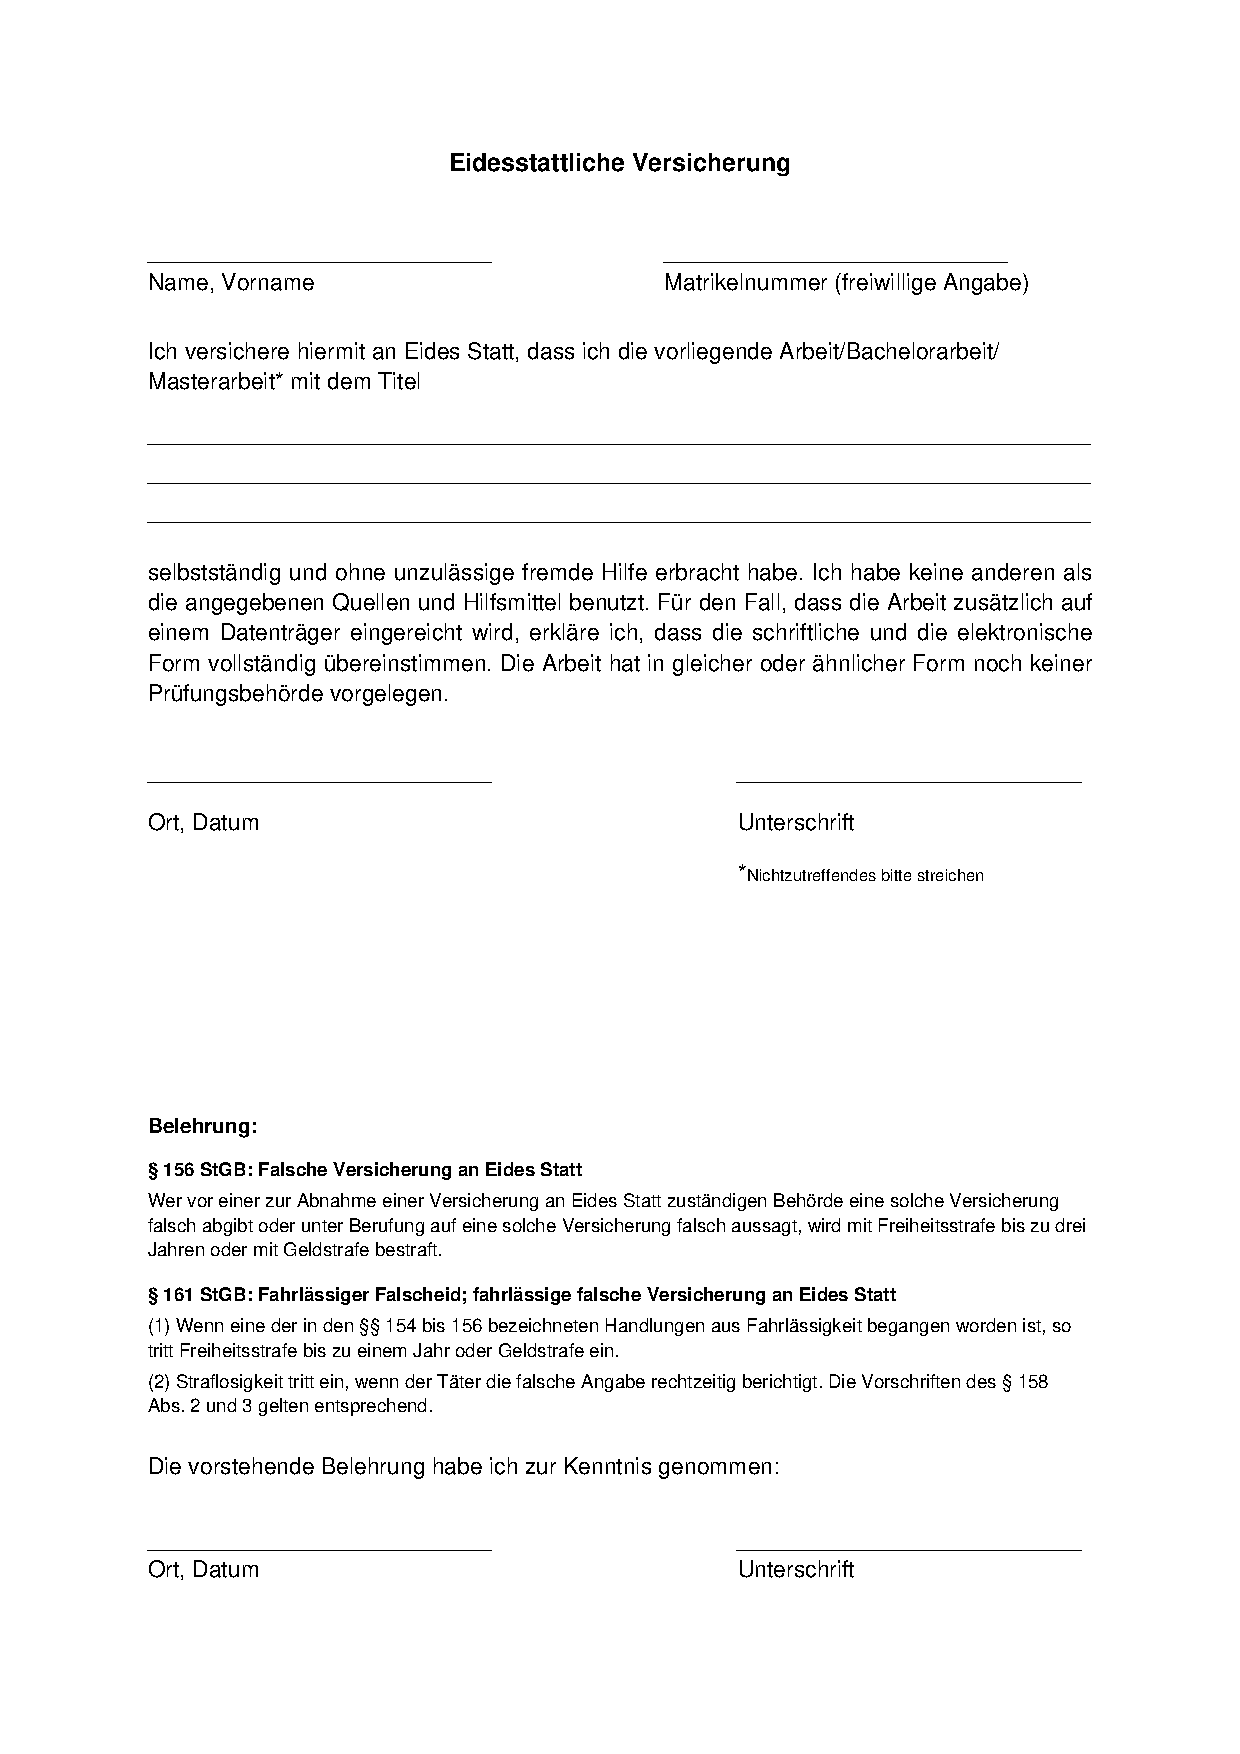
\includepdf{Formular_Eidesstattliche_Versicherung.pdf}

% Abstract
\begin{abstract}
This master thesis integrates the component bound branching rule, proposed by Vanderbeck et al. \cite{vanderbeck2010reformulation,vanderbeck1996exact}, into the branch-price-and-cut solver GCG. This rule, similarly to Vanderbeck's generic branching scheme \cite{vanderbeck2011branching}, exclusively operates within the Dantzig-Wolfe reformulated problem, where branching decisions generally have no corresponding actions in the original formulation. The current GCG framework requires modifications for such branching rules, especially within the pricing loop, as seen in Vanderbeck's method implementation. These rules also fail to utilize enhancements like dual value stabilization.

A significant contribution of this thesis is the enhancement of the GCG architecture to facilitate the seamless integration of new branching rules that operate solely on the reformulated problem. This allows these rules to benefit from current and future improvements in the branch-price-and-cut framework, including dual value stabilization, without necessitating alterations to the branching rule itself.

The thesis proposes an interface to manage constraints in the master problem that lack counterparts in the original formulation. These constraints require specific modifications to the pricing problems to ensure their validity in the master. The 'generic mastercut' interface, tightly integrated into the GCG solver, spans the pricing loop, column generation, and dual value stabilization. Enhancements to the existing branching rule interface complement this integration, enabling effective utilization of the generic mastercuts.

Finally, the component bound branching rule will be implemented using this new interface and evaluated on a set of benchmark instances. Its performance will be benchmarked against the existing Vanderbeck branching rule, offering a practical comparison of both approaches.
\end{abstract}
\cleardoublepage

% Table of contents
\tableofcontents
\cleardoublepage

% Chapters
\chapter{Introduction}
The development of efficient algorithms for solving large-scale mixed-integer programming (\MIP{}) problems has been a central focus of operations research for decades. Column generation, a powerful technique for solving large-scale linear programs, has been extended to integer programs through the branch-and-price algorithm. The effectiveness of branch-and-price relies heavily on the branching strategies employed and the ability to integrate various constraints into the reformulated problem during column generation.

In this thesis, we explore advanced branching rules and constraints within the context of the branch-and-price framework, particularly focusing on the implementation and evaluation of the component bound branching rule. This rule, as proposed by Desrosiers et al. \cite{thebook}, offers a simpler alternative to Vanderbeck's generic branching scheme \cite{vanderbeck2011branching} for branching on so-called component bound sequences \cite{vanderbeck1996exact}. As both branching rules operate entirely within the reformulated problem, integrating them into a branch-and-price framework requires careful consideration of the underlying mathematical structure and the implementation details.

The foundational concepts of polyhedron representation and the primal simplex algorithm are introduced in Chapter \ref{ch:preliminaries}, providing the mathematical and algorithmic background necessary for understanding the core methods discussed later. In Chapter \ref{ch:cg_bp}, we delve into the specifics of column generation and branch-and-price, detailing the algorithms and their implementation, including the Dantzig-Wolfe reformulation, which serves as the basis for the decomposition approach used in branch-and-price.

Chapter \ref{ch:tools} provides a brief overview of the \SCIP{} Optimization Suite, with a particular focus on the \GCG{} solver, which forms the foundation for the implementation work carried out in this thesis. In Chapter \ref{ch:cmpbnd}, we present the component bound branching rule in detail, including its separation procedure and a theoretical comparison to Vanderbeck's generic branching scheme.

One of the major contributions of this thesis is the introduction of a new interface within \GCG{} for handling constraints that exist solely within the master problem, termed \textbf{generic mastercuts}. These constraints, which do not have a direct counterpart in the original problem, require special handling within the solver, particularly with respect to synchronizing master variables across the search tree and applying dual value stabilization. Chapter \ref{ch:gm} begins by presenting the conceptual framework and definition of generic mastercuts, followed by an elaboration on the synchronization mechanisms and the application of dual value stabilization for these constraints, highlighting the technical innovations introduced in this thesis.

Chapter \ref{ch:implementation} focuses on the implementation aspects, detailing how the generic mastercut interface was integrated into \GCG{}, and how it supports the component bound branching rule.

The effectiveness of the component bound branching rule and the generic mastercut interface is rigorously evaluated in Chapter \ref{ch:evaluation}. We compare different separation heuristics and analyze the impact of dual value stabilization on the performance of the branching rule. Additionally, a detailed comparison with Vanderbeck's generic branching scheme provides insights into the conditions under which the component bound branching rule may offer advantages.

\cleardoublepage
\chapter{Preliminaries}\label{ch:preliminaries}

In this preliminary chapter we will provide a brief rundown of theorems and algorithms on which the techniques described in later chapters, such as Column Generation in Section \ref{sec:cg_bp_cg}, are building upon. Understanding these concepts is essential to understanding the theory later presented. If, however, one is familiar with these, we invite the reader to skip ahead to Chapter \ref{ch:cg_bp}.

\section{Polyhedron Representation}\label{sec:preliminaries_poly}
% Conic
\begin{definition}
Given $k$ points $\vec{x}_1, \dots, \vec{x}_k \in \mathbb{R}^n$, any $\vec{x} = \sum_{i=1}^{k} \alpha_i \vec{x}_i$ is a \textbf{conic combination} of the $\vec{x}_i$, iff $\forall i \in \{1, \dots, k\}. \alpha_i \geq 0$.
\end{definition}

% Convexity
\begin{definition}\label{def:convex}
Given $k$ points $\vec{x}_1, \dots, \vec{x}_k \in \mathbb{R}^n$, any $\vec{x} = \sum_{i=1}^{k} \alpha_i \vec{x}_i$ is a \textbf{convex combination} of the $\vec{x}_i$, iff $\sum_{i=1}^{k} \alpha_i = 1 \land \forall i \in \{1, \dots, k\}. \alpha_i \geq 0$.

The set of all convex combinations of $\vec{x}_1, \dots, \vec{x}_k$ is therefore defined as:

\begin{equation*}
\conv(\vec{x}_1, \dots, \vec{x}_k) \coloneqq \left\{\sum_{i=1}^{k} \alpha_i \vec{x}_i \mid \alpha_i \geq 0, i=1..k, \sum_{i=1}^{k} \alpha_i = 1\right\}
\end{equation*}
\end{definition}

\begin{corollary}\label{cor:intersection_convex}
The intersection of two convex sets is convex.
\end{corollary}

% Extreme Points
\begin{definition}
Let $\polyhedron{P}$ be a convex set. A point $\vec{p} \in \polyhedron{P}$ is an \textbf{extreme point} of $\polyhedron{P}$ if there is no non-trivial convex combination of any two points in $\polyhedron{P}$ expressing $\vec{p}$, i.e.:

\begin{equation*}
\forall \vec{x}_1, \vec{x}_2 \in \polyhedron{P}. \forall \alpha \in \left(0,1 \right). \vec{x}_1 \neq \vec{x}_2 \implies \vec{p} \neq \alpha \vec{x}_1 + (1 - \alpha) \vec{x}_2
\end{equation*}
\end{definition}

% Rays
\begin{definition}\label{def:rays}
Let $\polyhedron{P}$ be a convex set. A vector $\vec{r} \in \mathbb{R}_+^n \setminus \{0\}$ is a \textbf{ray} of $\polyhedron{P}$ iff $\forall \vec{x} \in \polyhedron{P}. \forall \beta \in \mathbb{R}_+. \vec{x} + \beta \vec{r} \in \polyhedron{P}$.

The cone of rays $\vec{r}_1, \dots, \vec{r}_k \in \mathbb{R}_+^n \setminus \{0\}$ is denoted as:

\begin{equation*}
\raycone(\vec{r}_1, \dots, \vec{r}_k) \coloneqq \left\{ \sum_{i=1}^{k} \alpha_i \vec{r}_i \mid \alpha_i \geq 0, i=1..k \right\}
\end{equation*}
\end{definition}

\begin{definition}
A ray $\vec{r}$ of $\polyhedron{P}$ is an \textbf{extreme ray} of $\polyhedron{P}$ if there is no non-trivial conic combination of any two rays in $\polyhedron{P}$ expressing $\vec{r}$, i.e.:

\begin{equation*}
\forall \vec{r}_1, \vec{r}_2 \in \polyhedron{P}. \forall \alpha_1, \alpha_2, \beta \in \mathbb{R}_+ \setminus \{0\}. \vec{r}_1 \neq \beta \vec{r}_2 \implies \vec{r} \neq \alpha_1 \vec{r}_1 + \alpha_2 \vec{r}_2
\end{equation*}
\end{definition}

% Hyperplane
\begin{definition}
A \textbf{hyperplane} $\polyhedron{H} \subset \mathbb{R}^n$ of a $n$-dimensional space is a subspace of dimension $n-1$, and can therefore be described using a vector $\vec{f} \in \mathbb{R}^n$ and a scalar $f \in \mathbb{R}$ as $\polyhedron{H} = \{\vec{x} \mid \vec{f}\transpose \vec{x} = f\}$.
\end{definition}

\begin{corollary}
Any hyperplane is a convex set.
\end{corollary}

\iffalse
\begin{proof}
Let $\polyhedron{H} = \{\vec{x} \mid \vec{f}\transpose \vec{x} = f\}$ be a hyperplane. Let $k \in \mathbb{N}$, $\vec{x}_1, \dots, \vec{x}_k \in \polyhedron{H}$. For any $\alpha_1, \dots, \alpha_k \in \mathbb{R}_+$ with $\sum_{i=1}^{k} \alpha_i = 1$:

\begin{align*}
\vec{f}\transpose \left( \sum_{i=1}^{k} \alpha_i \vec{x}_i \right)
&= \sum_{i=1}^{k} \alpha_i \vec{f}\transpose \vec{x}_i \\
&= \sum_{i=1}^{k} \alpha_i \cdot f \\
&= f \cdot \sum_{i=1}^{k} \alpha_i \\
&= f
\end{align*}

Therefore, the convex combination $\sum_{i=1}^{k} \alpha_i \vec{x}_i$ is in the hyperplane $\polyhedron{H}$.
\end{proof}
\fi

% Halfspace
\begin{definition}
A \textbf{halfspace} is the set either above or below a hyperplane. A halfspace is open if the points on the hyperplane are excluded; otherwise, it is closed.
\end{definition}

\begin{corollary}\label{cor:halfspace_convex}
Any halfspace is a convex set.
\end{corollary}

\iffalse
\begin{proof}
Let $\polyhedron{H}^+ = \{\vec{x} \mid \vec{f}\transpose \vec{x} > f\}$ be an open halfspace (analogous for $\polyhedron{H}^- = \{\vec{x} \mid \vec{f}\transpose \vec{x} < f\}$, and for the closed halfspaces). Let $k \in \mathbb{N}$, $\vec{x_1}, \dots, \vec{x_k} \in \polyhedron{H}^+$. For any $\alpha_1, \dots, \alpha_k \in \mathbb{R}_+$ with $\sum_{i=1}^{k} \alpha_i = 1$:

\begin{align*}
\vec{f}\transpose \left( \sum_{i=1}^{k} \alpha_i \vec{x}_i \right)
&= \sum_{i=1}^{k} \alpha_i \vec{f}\transpose \vec{x}_i \\
&> \sum_{i=1}^{k} \alpha_i \cdot f \\
&= f \cdot \sum_{i=1}^{k} \alpha_i \\
&= f
\end{align*}

Therefore, the convex combination $\sum_{i=1}^{k} \alpha_i \vec{x}_i$ is in the halfspace $\polyhedron{H}^+$.
\end{proof}
\fi

% Polyhedron
\begin{definition}
A \textbf{polyhedron} $\polyhedron{P} \subseteq \mathbb{R}^n$ is defined by the intersection of a set of closed halfspaces, i.e., $\polyhedron{P} \coloneqq \{\vec{x} \in \mathbb{R}^n \mid \mat{A} \vec{x} \geq \vec{b}\}$, with $\mat{A} \in \mathbb{R}^{m \times n}, \vec{b} \in \mathbb{R}^m$.
\end{definition}

\begin{corollary}
A polyhedron is a convex set.
\end{corollary}

\iffalse
\begin{proof}
Follows from Corollaries \ref{cor:intersection_convex} and \ref{cor:halfspace_convex}.
\end{proof}
\fi

% Monkowski-Weyl
\begin{definition}
The \textbf{Minkowski sum} of two sets $P, Q$ is defined by:
\begin{equation*}
P \oplus Q \coloneqq \left\{\vec{p} + \vec{q} \mid \vec{p} \in P \land \vec{q} \in Q \right\}
\end{equation*}
\end{definition}

\begin{theorem}[Minkowski-Weyl \cite{chappell2019minkowski,thebook}]\label{th:minkowski-weyl}
For $\polyhedron{P} \subseteq \mathbb{R}^n$ the following statements are equivalent:

\begin{enumerate}
\item $\polyhedron{P}$ is a polyhedron, i.e., there exists some finite matrix $\mat{A} \in \mathbb{R}^{m \times n}$ and some vector $\vec{b} \in \mathbb{R}^m$ such that $P = \{\vec{x} \in \mathbb{R}^n \mid \mat{A} \vec{x} \leq \vec{b}\}$
\item There exist fine vectors $\vec{v}_1, \dots, \vec{v}_s \in \mathbb{R}^n$ and finite vectors $\vec{r}_1, \dots, \vec{r}_t \in \mathbb{R}_+^n$, such that $P = \conv(\vec{v}_1, \dots, \vec{v}_s) \oplus \raycone(\vec{r}_1, \dots, \vec{r}_t)$
\end{enumerate}
\end{theorem}

In simple terms, the Minkowski-Weyl theorem states that any polyhedron can always be defined in two ways: either by its faces, i.e., closed halfspaces, or by its vertices and rays. Any polyhedron can be represented in this way using only its extreme points and extreme rays. Figure \ref{fig:minkowski-weyl} illustrates this theorem on two exemplary polyhedra.

\begin{figure}
\centering
\begin{tikzpicture}
% Define the extreme points
\coordinate (A) at (-4,0.5);
\coordinate (B) at (-5,2);
\coordinate (C) at (-4,3);
\coordinate (D) at (-3,3);
\coordinate (E) at (-3,0);

% Draw the filled region
\fill[fill=blue!30] (A) -- (B) -- (C) -- (D) -- (E) -- cycle;

% Draw the extreme points
\foreach \point in {A, B, C, D, E}
  \fill[black] (\point) circle (2pt);

% Draw the edges of the polyhedron
\draw[thick] (A) -- (B) -- (C) -- (D) -- (E) -- cycle;

%%%%%%%%%%

% Define the extreme points
\coordinate (A) at (1,2);
\coordinate (B) at (0,0);
\coordinate (C) at (2,1);

% Define the ends of the rays
\path (A) -- +(45:2cm) coordinate (A-ray);
\path (C) -- +(45:2cm) coordinate (C-ray);
\path (A) -- +(45:1cm) coordinate (A-ray-short);
\path (C) -- +(45:1cm) coordinate (C-ray-short);

% Draw the filled region
\fill[fill=blue!30] (A) -- (B) -- (C) -- (C-ray) -- (A-ray) -- cycle;

% Draw the extreme points
\foreach \point in {A, B, C}
  \fill[black] (\point) circle (2pt);

% Draw the edges of the polyhedron
\draw[thick] (A) -- (B) -- (C);

% Draw rays from points (1,2) and (2,1)
\draw[dashed, thick, gray!80, -latex] (A) -- (A-ray); % Ray at 45 degrees from point (1,2)
\draw[dashed, thick, gray!80, -latex] (C) -- (C-ray); % Ray at 45 degrees from point (2,1)
\draw[thick, red, -latex] (A) -- (A-ray-short); % Ray at 45 degrees from point (1,2)
\draw[thick, red, -latex] (C) -- (C-ray-short); % Ray at 45 degrees from point (2,1)
\end{tikzpicture}
\caption{Illustration of the Minkowski-Weyl theorem. The left figure shows a polytope represented by its extreme points. Unbounded polyhedra, such as the one on the right, require extreme rays, shown in red, for a complete description.}
\label{fig:minkowski-weyl}
\end{figure}

The following theorem builds upon the Minkowski-Weyl theorem to describe a polyhedron, which is represented by its extreme points $\{\vec{x}_p\}_{p \in P}$ and extreme rays $\{\vec{x}_r\}_{r \in R}$, using hyperplanes. Here, the sets $P, R$ are used to index the extreme points and extreme rays, respectively.

\begin{theorem}[Nemhauser-Wolsey \cite{wolsey2014integer,thebook}]\label{th:nemhauser-wolsey}
Consider the polyhedron $\polyhedron{P} = \{\vec{x} \in \mathbb{R}^n \mid \mat{Q} \vec{x} \geq \vec{b}\}$ with full row rank matrix $\mat{Q} \in \mathbb{R}^{m \times n}$, i.e., $\rank(\mat{Q}) = m \leq n \land \polyhedron{P} \neq \emptyset$.

An equivalent description of $\polyhedron{P}$ using its extreme points $\{\vec{x}_p\}_{p \in P}$ and extreme rays $\{\vec{x}_r\}_{r \in R}$ is:

\begin{equation}
\polyhedron{P} = \left\{ \vec{x} \in \mathbb{R}^n \middle\vert
\begin{aligned}
\sum_{p \in P} \vec{x}_p \lambda_p &+ &\sum_{r \in R} \vec{x}_r \lambda_r &= \vec{x} &\\
\sum_{p \in P} \lambda_p & & &= 1 &\\
\lambda_p & & &\geq 0 &\forall p \in P\\
& &\lambda_r &\geq 0 &\forall r \in R
\end{aligned}
\right\}
\end{equation}
\end{theorem}

The conditions of the Minkowski-Weyl theorem are clearly encoded in the Nemhauser-Wolsey theorem: the second and third lines ensure that the convex set of the extreme points is considered in the first line (Definition \ref{def:convex}), the last pertains to the cone of extreme rays (Definition \ref{def:rays}), and the first line represents the Minkowski sum of the convex hull of extreme rays and the cone of extreme rays.

By requiring $\vec{x} \in \mathbb{Z}^n$ in Theorem \ref{th:nemhauser-wolsey}, we can also describe the integral polyhedra using possibly fractional extreme points and rays. Alternatively, the Nemhauser-Wolsey theorem has been adapted to describe integral polyhedra using only integral (interior) points and (integer-scaled) extreme rays, as shown in the following theorem.

\begin{theorem}[Nemhauser-Wolsey \cite{wolsey2014integer,thebook}]\label{th:nemhauser-wolsey-integer}
Consider the polyhedron $\polyhedron{P} = \{\vec{x} \in \mathbb{R}^n \mid \mat{Q} \vec{x} \geq \vec{b}\}$ with full row rank matrix $\mat{Q} \in \mathbb{R}^{m \times n}$, i.e., $\rank(\mat{Q}) = m \leq n \land \polyhedron{P} \neq \emptyset$. Have $\polyhedron{Q} \coloneqq \polyhedron{P} \cap \mathbb{Z}^n \neq \emptyset$ be the integer hull of $\polyhedron{P}$.

An equivalent description of $\polyhedron{Q}$ using a finite subset $\{\vec{x}_p\}_{p \in \ddot{P}}$ of its integer points and its (integer-scaled) extreme rays $\{\vec{x}_r\}_{r \in R}$ is:

\begin{equation}
\polyhedron{Q} = \left\{ \vec{x} \in \mathbb{Z}^n \middle\vert
\begin{aligned}
\sum_{p \in \ddot{P}} \vec{x}_p \lambda_p &+ &\sum_{r \in R} \vec{x}_r \lambda_r &= \vec{x} &\\
\sum_{p \in \ddot{P}} \lambda_p & & &= 1 &\\
\lambda_p & & &\in \{0, 1\} &\forall p \in \ddot{P}\\
& &\lambda_r &\in \mathbb{Z}_+ &\forall r \in R
\end{aligned}
\right\}
\end{equation}
\end{theorem}

\begin{note}\label{note:nemhauser-wolsey}
A notable difference between the Nemhauser-Wolsey theorem for real polyhedra and integral polyhedra is that for the former it suffices to use extreme points and extreme rays, while for the latter, interior points of $\polyhedron{Q}$ might be required to describe the integer hull $\polyhedron{Q}$.
\end{note}

\section{Primal Simplex Algorithm}\label{sec:preliminaries_psa}
Have the following linear program in standard form:
\begin{equation}\label{eq:lp_standard}
\begin{aligned}
&\min & \vec{c}\transpose \vec{x} & & \\
&\st & \mat{A} \vec{x} & = \vec{b} & \left[\vec{\pi}\right] \\
&& \vec{x} & \geq \vec{0} &
\end{aligned}
\end{equation}

The primal simplex algorithm finds an optimal solution by moving from one extreme point of the polyhedron to the next, therefore always remaining feasible. A central part of this algorithm is the sufficient optimality condition. For a basic solution $\vec{X} = \left[\vec{x}_\indexset{B}, \vec{x}_\indexset{N}\right]$ at a given extreme point to be optimal, the reduced costs $\bar{c}_j \coloneqq c_j - \vec{\pi}\transpose \vec{a}_j$ for $j \in \indexset{N}$ must be non-negative.

This sufficient optimality condition gives rise to the \textbf{pricing problem}, which either verifies the optimality of the current basic solution, and otherwise determines the non-basic variable $x_l$, $l \in \indexset{N}$ with the least reduced cost ($\bar{c}_l < 0$) to be swapped into the basis next, according to Dantzig's rule (TODO cite). Formally, this can be written as:
\begin{equation}
l \in \underset{j \in \indexset{N}}{\arg\min} \, c_j - \vec{\pi}\transpose \vec{a}_j
\end{equation}
or as the linear program:
\begin{equation}\label{eq:psa_pp}
\bar{c}(\vec{\pi}) = \underset{j \in \indexset{N}}{\min} \, c_j - \vec{\pi}\transpose \vec{a}_j
\end{equation}

Solving the pricing problem thus plays an integral role in the primal simplex algorithm:

\begin{algorithm}
\caption{Primal simplex algorithm with Dantzig's rule}
\KwIn{\LP{} in standard form (\ref{eq:lp_standard}); Basic and non-basic index-sets $\indexset{B},\indexset{N}$}
\KwOut{Optimal Solution $(\vec{x}, z)$}
\Loop{
	$\vec{\pi}\transpose \gets \vec{c}_\indexset{B}\transpose \mat{A}_\indexset{B}^{-1}$;
	$\bar{\vec{b}} \gets \mat{A}_\indexset{B}^{-1} \vec{b}$\;
	$\bar{c}_j \gets c_j - \vec{\pi}\transpose \vec{a}_j$;$ \qquad \forall j \in \indexset{N}$\\
	$l \gets \underset{j \in \indexset{N}}{\arg\min} \, \bar{c}_j$;
	$\bar{c}(\vec{\pi}) \gets \bar{c}_l$\;
	\If{$\bar{c}(\vec{\pi}) \geq 0$}{
		\Return{$\left(\left[\bar{\vec{b}}, \vec{0}\right], \vec{c}_\indexset{B}\transpose \vec{x}_\indexset{B}\right)$} \textit{by optimality}
	}
	$\bar{\vec{a}}_l \gets \mat{A}_\indexset{B}^{-1} \vec{a}_l$\;
	\If{$\bar{\vec{a}}_l \leq \vec{0}$}{
		\Return{\None} \textit{by unboundedness}
	}
	$s \gets \underset{i \in \{1, \dots, m\}}{\arg\min} \, \frac{\bar{b}_i}{\bar{a}_{il}}$;
	$x_l \gets \frac{\bar{b}_s}{\bar{a}_{sl}}$;
	$\indexset{B} \gets \indexset{B} \cup \{l\} \subseteq \{s\}$;
	$\indexset{N} \gets \indexset{N} \cup \{s\} \subseteq \{l\}$\;
}
\end{algorithm}

\cleardoublepage
\chapter{Column Generation and Branch-and-Price}\label{ch:cg_bp}

\section{Column Generation}\label{sec:cg_bp_cg}
Let us consider the following linear program, which we will henceforth call the \textbf{master problem} \MP{}, where $c_\vec{x} \in \mathbb{R}, \vec{a}_\vec{x}, \vec{b} \in \mathbb{R}^m, \forall \vec{x} \in \indexset{X}$:
\begin{equation}
\begin{aligned}
z_\MP{} = &\min & \sum_{\vec{x} \in \indexset{X}} c_\vec{x} \lambda_\vec{x} & & & \\
&\st & \sum_{\vec{x} \in \indexset{X}} \vec{a}_\vec{x} \lambda_\vec{x} & \geq \vec{b} & \left[\vec{\pi}\right] & \\
&& \lambda_\vec{x} & \geq \vec{0} & & \forall \vec{x} \in \indexset{X}
\end{aligned}
\end{equation}
Assume the number of variables is huge, i.e. a lot larger than the number of constraints ($m \ll \abs{\indexset{X}} < \infty$). Because of this, solving \MP{} in a reasonable amount of time, sometimes at all, is infeasible.

We can, however, make use of a crucial property of the primal simplex algorithm: at any given vertex solution, only few variables are in the basis. Most variables are in the non-basis, and therefore have a solution value of $0$. Having a solution value of $0$ is equivalent to not being in the linear program at all. Therefore, the primal simplex algorithm can also function using a manageable subset of variables $\indexset{X}' \subseteq \indexset{X}$, finding a possibly non-optimal, yet still feasible solution for the entire optimization problem \MP{}. We denote this master problem restricted to a subset of variables as the \textbf{restricted master problem} \RMP{}:
\begin{equation}
\begin{aligned}
z_\RMP{} = &\min & \sum_{\vec{x} \in \indexset{X}'} c_\vec{x} \lambda_\vec{x} & & & \\
&\st & \sum_{\vec{x} \in \indexset{X}'} \vec{a}_\vec{x} \lambda_\vec{x} & \geq \vec{b} & \left[\vec{\pi}\right] & \\
&& \lambda_\vec{x} & \geq \vec{0} & & \forall \vec{x} \in \indexset{X}'
\end{aligned}
\end{equation}

Assuming \MP{} is feasible, two important aspects of finding an optimal solution to \MP{} are still missing: first, how do we find a subset $\indexset{X}'$ of the variables, such that \RMP{} stays feasible? Without this property of the set of variables, no solution of \RMP{} can be found, and therefore none can be found for \MP{}, which would contradict the feasibility of \MP{}. Secondly, assuming a solution of \RMP{} was found, possibly even optimal within \RMP{}, how could we build upon this solution to eventually find an optimal solution for \MP{}?

In the following we will dive into these two questions in detail (Sections \ref{sec:cg_bp_cg_farkas} and \ref{sec:cg_bp_cg_reduced}), making way for the final column generation algorithm (Section \ref{sec:cg_bp_cg_alg}).

\subsection{Farkas Pricing}\label{sec:cg_bp_cg_farkas}
Let us assume \MP{} is feasible, but our current selection of variables $\indexset{X}' \subset \indexset{X}$ results in the \RMP{} being infeasible. The task is now to find additional variables such that a new set $\indexset{X}''$ with $\indexset{X}' \subset \indexset{X}'' \subseteq \indexset{X}$ makes the \RMP{} feasible. For this, consider Farkas' lemma:

\begin{theorem}[Farkas' lemma]\label{th:farkas_lemma}
Given $\mat{A} \in \mathbb{R}^{m \times n}$ and $\vec{b} \in \mathbb{R}^m$, then exactly one of the following statements holds:
\begin{enumerate}
	\item $\exists \vec{x} \in \mathbb{R}_+^n. \, \mat{A} \vec{x} \geq \vec{b}$
	\item $\exists \vec{\pi} \in \mathbb{R}_+^n. \, \vec{\pi}\transpose \mat{A} \leq \vec{0} \land \vec{\pi}\transpose \vec{b} > 0$
\end{enumerate}
\end{theorem}

Given that the \MP{} is feasible, the following must hold for the \MP{} with $\mat{A} = \mat{A}_{\vert \indexset{X}}$:
\begin{equation}
\begin{aligned}
& \exists \vec{x} \in \mathbb{R}_+^n. \, \mat{A} \vec{x} \geq \vec{b} \qquad \land \neg \exists \vec{\pi} \in \mathbb{R}_+^n. \, \vec{\pi}\transpose \mat{A} \leq \vec{0} \land \vec{\pi}\transpose \vec{b} > 0 \\
\Leftrightarrow & \exists \vec{x} \in \mathbb{R}_+^n. \, \mat{A} \vec{x} \geq \vec{b} \qquad \land \forall \vec{\pi} \in \mathbb{R}_+^n. \, \neg \left( \vec{\pi}\transpose \mat{A} \leq \vec{0} \land \vec{\pi}\transpose \vec{b} > 0 \right)\\
\Leftrightarrow & \exists \vec{x} \in \mathbb{R}_+^n. \, \mat{A} \vec{x} \geq \vec{b} \qquad \land \forall \vec{\pi} \in \mathbb{R}_+^n. \, \vec{\pi}\transpose \mat{A} > \vec{0} \lor \vec{\pi}\transpose \vec{b} \leq 0 \\
\Rightarrow & \exists \vec{x} \in \mathbb{R}_+^n. \, \exists \vec{\pi} \in \mathbb{R}_+^n. \, \vec{\pi}\transpose \mat{A} \vec{x} \geq \vec{\pi}\transpose \vec{b}
\end{aligned}
\end{equation}

Furthermore, from the infeasibility of \RMP{} we can also derive the following statement:
\begin{equation}
\begin{aligned}
& \left( \forall \vec{\pi} \in \mathbb{R}_+^n. \, \vec{\pi}\transpose \mat{A} > \vec{0} \lor \vec{\pi}\transpose \vec{b} \leq 0 \right) \land \left( \exists \vec{\pi} \in \mathbb{R}_+^n. \, \vec{\pi}\transpose \mat{A}_{\vert \indexset{X}'} \leq \vec{0} \land \vec{\pi}\transpose \vec{b} > 0 \right) \\
\Rightarrow & \left( \neg \forall \vec{\pi} \in \mathbb{R}_+^n. \, \vec{\pi}\transpose \vec{b} \leq 0 \right) \land \left( \exists \vec{\pi} \in \mathbb{R}_+^n. \, \vec{\pi}\transpose \mat{A}_{\vert \indexset{X}'} > \vec{0} \right)
\end{aligned}
\end{equation}

Therefore, there is some variable $\vec{x} \in \indexset{X} \setminus \indexset{X}'$ such that its column $\vec{a}_\vec{x} \coloneqq \mat{A}_{\vert \{\vec{x}\}}$ is $\vec{\pi}\transpose \vec{a}_\vec{x} > 0$ for some $\vec{\pi} \in \mathbb{R}_+^n$.

This process of finding corresponding columns $\vec{a}_\vec{x}$ to add to the \RMP{} can be formalized as a pricing problem with cost coefficients $c_\vec{x} = 0$:
\begin{equation}
\operatorname{F}(\vec{\pi}) = \underset{x \in \indexset{X}}{\min} \, -\vec{\pi}\transpose \vec{a}_x
\end{equation}

We can add all solutions $\vec{x}$ with a solution value of $\operatorname{F}(\vec{\pi}) > 0$ to $\indexset{X}'' \coloneqq \indexset{X}' \cup \{\vec{x}_i\}$, thus turning any infeasible \RMP{} feasible.

\subsection{Reduced Cost Pricing}\label{sec:cg_bp_cg_reduced}

\subsection{Column Generation Algorithm}\label{sec:cg_bp_cg_alg}


\section{Dantzig-Wolfe Reformulation}\label{sec:cg_bp_dwr}
The column generation algorithm presented in Section \ref{sec:cg_bp_cg} is particularly useful when we can directly formulate our optimization problem using a master and a pricing problem. However, many problems are provided in the general form of a \LP{}. Using the Dantzig-Wolfe reformulation, we can transform such a \LP{} into a master and pricing problem, making it suitable for column generation \cite{thebook}. This section introduces this technique and demonstrates how it can be applied to solve a \LP{}.

\begin{equation}
\begin{aligned}
z^*_\LP{} = &\min & \vec{c}\transpose \vec{x} & & & \\
&\st & \mat{A} \vec{x} & \geq \vec{b} & \left[\vec{\sigma}_\vec{b}\right] & \\
&& \mat{D} \vec{x} & \geq \vec{d} & \left[\vec{\sigma}_\vec{d}\right] & \\
&& \vec{x} & \geq \vec{0}
\end{aligned}
\end{equation}

Consider the above \LP{}. The solution space defined by its constraints can be viewed as the intersection of the following two polyhedra:

\begin{equation}
\begin{aligned}
\polyhedron{A} &\coloneqq \left\{ \vec{x} \geq \vec{0} \mid \mat{A} \vec{x} \geq \vec{b} \right\} &\neq \emptyset \\
\polyhedron{D} &\coloneqq \left\{ \vec{x} \geq \vec{0} \mid \mat{D} \vec{x} \geq \vec{d} \right\} &\neq \emptyset
\end{aligned}
\end{equation}

Applying the Nemhauser-Wolsey Theorem (Theorem \ref{th:nemhauser-wolsey}) on polyhedron $\polyhedron{D}$, we can reformulate the \LP{} using $\polyhedron{D}$'s extreme points $\{\vec{x}_p\}_{p \in P}$ and extreme rays $\{\vec{x}_r\}_{r \in R}$. To achieve this, we substitute the original variables $\vec{x}$ with these extreme points and extreme rays using:

\begin{equation}
\begin{aligned}
\vec{x} &= \sum_{p \in P} \vec{x}_p \lambda_p + \sum_{r \in R} \vec{x}_r \lambda_r \\
\vec{c}\transpose \vec{x} &= \sum_{p \in P} \vec{c}\transpose \vec{x}_p \lambda_p + \sum_{r \in R} \vec{c}\transpose \vec{x}_r \lambda_r \\
\mat{A} \vec{x} &= \sum_{p \in P} \mat{A} \vec{x}_p \lambda_p + \sum_{r \in R} \mat{A} \vec{x}_r \lambda_r
\end{aligned}
\end{equation}

Using the following shorthand notations:

\begin{equation}
\begin{aligned}
c_p &\coloneqq \vec{c}\transpose \vec{x}_p
&c_r &\coloneqq \vec{c}\transpose \vec{x}_r \\
\vec{a}_p &\coloneqq \mat{A} \vec{x}_p
&\vec{a}_r &\coloneqq \mat{A} \vec{x}_r
\end{aligned}
\end{equation}

We obtain a new \MP{} equivalent to the \LP{}:

\begin{equation}
\begin{aligned}
z^*_\MP{} = &\min & \sum_{p \in P} c_p \lambda_p &+ &\sum_{r \in R} c_r \lambda_r & & & \\
&\st & \sum_{p \in P} \vec{a}_p \lambda_p &+ &\sum_{r \in R} \vec{a}_r \lambda_r & \geq \vec{b} & \left[\vec{\pi}_\vec{b}\right] \\
&& \sum_{p \in P} \lambda_p & & & = 1 & \left[\pi_0 \right] & \\
&& \lambda_p & & & \geq 0 & & \forall p \in P \\
&& & & \lambda_r & \geq 0 & & \forall r \in R \\
&& \sum_{p \in P} \vec{x}_p \lambda_p &+ &\sum_{r \in R} \vec{x}_r \lambda_r & = \vec{x} \geq \vec{0} & &
\end{aligned}
\end{equation}

In this formulation, the last constraint corresponds to projecting a solution of the \MP{} using the $\lambda$ variables back into a solution of the original \LP{}. As this constraint is not otherwise involved in the optimization, it is often omitted during the solving stages and only used afterward to reconstruct a solution using the original $\vec{x}$ variables \cite{thebook}.

Since the extreme points and extreme rays of $\polyhedron{D}$ are often unknown, and their number might be enormous, solving the \MP{} directly is typically infeasible \cite{thebook}. Instead, we can generate these columns iteratively using column generation. For this, we need a subproblem that finds (improving) columns for the \MP{}, i.e., extreme points and extreme rays of $\polyhedron{D}$. We can formulate this pricing problem as follows:

\begin{equation}
\begin{aligned}
z^*_\SP{} = &\min & \left( \vec{c}\transpose - \vec{\pi}_\vec{b}\transpose \mat{A} \right) \vec{x} - \pi_0 & & \\
&\st & \mat{D} \vec{x} & \geq \vec{d} & \left[\vec{\pi}_\vec{d}\right] \\
&& \vec{x} & \geq \vec{0}
\end{aligned}
\end{equation}

We start by solving the \RMP{} using a subset of the extreme points $P' \subset P$ and extreme rays $R' \subset R$, yielding the dual values $\vec{\pi}_\vec{b}$ and $\pi_0$ for the \SP{}. Solving this \SP{} to optimality then leads to a solution $\vec{x}^*$ with objective value $z^*_\SP{}$. The value of $z^*_\SP{}$ determines whether we add a column to \RMP{}, and if so, which column to add:

\begin{itemize}
\item If $-\infty < z^*_\SP{} < 0$, $\vec{x}^*$ is an extreme point $\vec{x}_p, p \in P \setminus P'$, and we add column $\begin{bmatrix} \vec{c}\transpose \vec{x}^* \\ \mat{A} \vec{x}^* \\ 1 \end{bmatrix}$ to \RMP{}.
\item If $z^*_\SP{} = -\infty$, $\vec{x}^*$ is an extreme ray $\vec{x}_r, r \in R \setminus R'$, and we add column $\begin{bmatrix} \vec{c}\transpose \vec{x}^* \\ \mat{A} \vec{x}^* \\ 0 \end{bmatrix}$ to \RMP{}.
\item If $z^*_\SP{} \geq 0$, there exists no improving column for \RMP{}, and the column generation algorithm terminates.
\end{itemize}

While theoretically, the grouping of constraints in the original \LP{} formulation for the Dantzig-Wolfe reformulation does not change the optimal solution, in practice, the choice of grouping can significantly impact the performance of the column generation algorithm. Since many iterations of the column generation algorithm are often required to find an optimal solution, ideally, one wants \SP{} to be efficiently solvable. Numerous efficient algorithms for specific optimization problems exist, and by grouping constraints in a way that \SP{} corresponds to such structures, one can leverage these algorithms to solve \SP{} efficiently \cite{thebook}. Although there are ways to find such groupings automatically, this topic is beyond the scope of this thesis.

\section{Dantzig-Wolfe Reformulation for Integer Programs}\label{sec:cg_bp_ip}
Dantzig-Wolfe reformulation can also be applied to integer programs. In this section, we will show how to reformulate an integer program into a master and pricing problem, specifically focusing on the integrality conditions. Later, in Section \ref{sec:cg_bp_bp}, we will explore how to solve such an integer program using column generation.

Consider the following integer program:
\begin{equation}
\begin{aligned}
z^*_\IP{} = &\min & \vec{c}\transpose \vec{x} & & & \\
&\st & \mat{A} \vec{x} & \geq \vec{b} & \left[\vec{\sigma}_\vec{b}\right] & \\
&& \mat{D} \vec{x} & \geq \vec{d} & \left[\vec{\sigma}_\vec{d}\right] & \\
&& \vec{x} & {\color{blue} \in \mathbb{Z}_ +^n}
\end{aligned}
\end{equation}

Again, we group the constraints into two sets:
\begin{equation}
\begin{aligned}
\polyhedron{A} &\coloneqq \left\{ \vec{x} {\color{blue} \in \mathbb{Z}^n} \mid \mat{A} \vec{x} \geq \vec{b} \right\} &\neq \emptyset \\
\polyhedron{D} &\coloneqq \left\{ \vec{x} {\color{blue} \in \mathbb{Z}^n} \mid \mat{D} \vec{x} \geq \vec{d} \right\} &\neq \emptyset
\end{aligned}
\end{equation}
Note that $\polyhedron{A}$ and $\polyhedron{D}$ are now the integer hulls of the original polyhedra. For simplicity, let us denote the convex hulls defined by both groups of constraints as:
\begin{equation}
\begin{aligned}
\polyhedron{A}' &\coloneqq \left\{ \vec{x} \geq \vec{0} \mid \mat{A} \vec{x} \geq \vec{b} \right\} &\neq \emptyset \\
\polyhedron{D}' &\coloneqq \left\{ \vec{x} \geq \vec{0} \mid \mat{D} \vec{x} \geq \vec{d} \right\} &\neq \emptyset
\end{aligned}
\end{equation}

There are two ways to proceed from here. The straightforward approach, called \textbf{Convexification}, follows the method seen in the Dantzig-Wolfe reformulation of linear programs, retaining the integrality constraints on $\vec{x}$ in both the master and pricing problem. Alternatively, in \textbf{Discretization}, we modify our approach slightly, adding integrality constraints to the master variables to ensure the integrality of the original variables.

\subsection{Convexification}\label{sec:cg_bp_ip_convexification}
As seen in Section \ref{sec:cg_bp_dwr}, we can reformulate the polyhedron $\polyhedron{D}$, which is now the integer hull defined by the constraints $\mat{D} \vec{x} \geq \vec{d}$, using the Nemhauser-Wolsey Theorem (Theorem \ref{th:nemhauser-wolsey}). This results in a master problem where the original variables $\vec{x}$ are represented as a convex combination of extreme points and extreme rays of $\polyhedron{D}$:

\begin{equation}
\begin{aligned}
z^*_\MP{} = &\min & \sum_{p \in P} c_p \lambda_p &+ &\sum_{r \in R} c_r \lambda_r & & & \\
&\st & \sum_{p \in P} \vec{a}_p \lambda_p &+ &\sum_{r \in R} \vec{a}_r \lambda_r & \geq \vec{b} & \left[\vec{\pi}_\vec{b}\right] \\
&& \sum_{p \in P} \lambda_p & & & = 1 & \left[\pi_0 \right] & \\
&& \lambda_p & & & \geq 0 & & \forall p \in P \\
&& & & \lambda_r & \geq 0 & & \forall r \in R \\
&& \sum_{p \in P} \vec{x}_p \lambda_p &+ &\sum_{r \in R} \vec{x}_r \lambda_r & = \vec{x} {\color{blue} \in \mathbb{Z}_+^n} & &
\end{aligned}
\end{equation}

In contrast to the Dantzig-Wolfe reformulation for linear programs, during convexification the last constraint, which reconstructs an original solution using a solution of the master problem, is crucial during the solving process to ensure the integrality of the original variables and cannot simply be computed after a solution has been found. The master problem has the following pricing subproblem:

\begin{equation}
\begin{aligned}
z^*_\SP{} = &\min & \left( \vec{c}\transpose - \vec{\pi}_\vec{b}\transpose \mat{A} \right) \vec{x} - \pi_0 & & \\
&\st & \mat{D} \vec{x} & \geq \vec{d} & \left[\vec{\pi}_\vec{d}\right] \\
&& \vec{x} & {\color{blue} \in \mathbb{Z}_+^n}
\end{aligned}
\end{equation}

These two changes marked in blue are the key differences between the Dantzig-Wolfe reformulation of linear programs and integer programs, ensuring that we find integer solutions for our original problem.

The beauty of this approach lies in the fact that the subproblem only generates the extreme points and extreme rays of the integer hull of $\{\vec{x} \geq \vec{0} \mid \mat{D} \vec{x} \geq \vec{d}\}$, regardless of how well the constraints $\mat{D} \vec{x} \geq \vec{d}$ approximate this integer hull. Therefore, we implicitly make use of the integer hull of $\polyhedron{D}$ without explicitly defining it.

$\lambda$ solutions to the \MP{} might lead to fractional $\vec{x}$ solutions. In this case, we must branch on those fractional original variables \cite{thebook}. We will discuss this in more detail in Section \ref{sec:cg_bp_bp_branching_original}.

\subsection{Discretization}\label{sec:cg_bp_ip_discretization}
In the discretization approach, we use the adaptation of the Nemhauser-Wolsey Theorem to integer polyhedra (Theorem \ref{th:nemhauser-wolsey-integer}) to reformulate the polyhedron $\polyhedron{D}$, yielding the following master problem:

\begin{equation}
\begin{aligned}
z^*_\MP{} = &\min & \sum_{p \in \ddot{P}} c_p \lambda_p &+ &\sum_{r \in R} c_r \lambda_r & & & \\
&\st & \sum_{p \in \ddot{P}} \vec{a}_p \lambda_p &+ &\sum_{r \in R} \vec{a}_r \lambda_r & \geq \vec{b} & \left[\vec{\pi}_\vec{b}\right] \\
&& \sum_{p \in \ddot{P}} \lambda_p & & & = 1 & \left[\pi_0 \right] & \\
&& \lambda_p & & & \in \{0, 1\} & & \forall p \in \ddot{P} \\
&& & & \lambda_r & \in \mathbb{Z}_+ & & \forall r \in R \\
&& \sum_{p \in \ddot{P}} \vec{x}_p \lambda_p &+ &\sum_{r \in R} \vec{x}_r \lambda_r & = \vec{x} {\color{blue} \in \mathbb{Z}_+^n} & &
\end{aligned}
\end{equation}

By design, a solution to the master problem is now guaranteed to be transformable into an integer solution of the original problem. Therefore, the last constraint can be omitted during the solving process. Solving the linear relaxation of the \RMP{} might lead to fractional $\lambda$ variables, which we can then branch on \cite{thebook}. Keeping in mind that $\ddot{P}$ is a subset of integer points of $\polyhedron{D}$, i.e., it might include interior points, we must find a pricing problem that can generate not only extreme points (and rays) of $\polyhedron{D}$ but also interior points. This, however, is not trivial, since mathematical optimization typically focuses on finding the most optimal solutions, i.e., the extreme points. We can postpone this concern for now and use the same pricing problem as in the convexification approach:

\begin{equation}
\begin{aligned}
z^*_\SP{} = &\min & \left( \vec{c}\transpose - \vec{\pi}_\vec{b}\transpose \mat{A} \right) \vec{x} - \pi_0 & & \\
&\st & \mat{D} \vec{x} & \geq \vec{d} & \left[\vec{\pi}_\vec{d}\right] \\
&& \vec{x} & {\color{blue} \in \mathbb{Z}_+^n}
\end{aligned}
\end{equation}

As we will discuss in Section \ref{sec:cg_bp_bp_branching_master}, the concern of generating interior points is addressed during the branching process, allowing us to generate such points on the fly. Therefore, combined with branching, the discretization approach is also a viable method to solve integer programs using column generation.

\section{Branch-and-Price}\label{sec:cg_bp_bp}
In Section \ref{sec:cg_bp_ip} we have seen how to reformulate an integer program into a master and pricing problem, specifically focusing on the integrality conditions. In this section, we will dive into how we then solve such an integer master program using column generation. First, let us remember what branching is for. Recall, that often we cannot solve an integer problem directly. Instead, we rely on the \LP{} relaxations of the problem which in turn can be solved by algorithms such as the simplex method. An optimal solution of the \LP{} relaxation might have some fractional values for the integer variables, i.e. produce infeasible solutions for the \IP{}. To overcome this, we branch on these fractional variables, creating subproblems, which explicitly cut off these fractional solutions. By recursively solving these subproblems, we eventually find an optimal integer solution. This process is widely known as \textbf{branch-and-bound}.

In the context of column generation for integer master programs, we proceed similarly: first, we relax the integrality constraints of the master problem, which allows us to solve the relaxation using column generation to optimality. Then, we check if the integrality conditions are satisfied. If not, we must cut off the fractional solution by branching. Combining branching with column generation, we obtain the term \textbf{branch-and-price}.

We have gotten to know two distinct approaches of reformulating an \IP{} into a (integer) master and pricing problem: convexification (Section \ref{sec:cg_bp_ip_convexification}) and discretization (Section \ref{sec:cg_bp_ip_discretization}). Since we require integrality of the original variables in both approaches, it is always possible to branch on fractional solutions of the original variables. We have seen, however, that discretization additionally introduces integrality constraints on the master variables which in turn imply integrality of the original variables. Therefore, in discretization, we can branch on the master variables as well. In the following, we will discuss both approaches in more detail.

\subsection{Branching on the Original Variables}\label{sec:cg_bp_bp_branching_original}
Assume we have a fractional solution $\vec{x}_\MP{}^*$ to the relaxed restricted master problem \RMP{}, i.e. there is some $x_j^* \not\in \mathbb{Z}$ for some integer variable $x_j$. Then we can cut off this fractional solution by creating two subbranches (\textbf{dichotomous branching}), one where $x_j \leq \floor{x_j^*}$ and one where $x_j \geq \ceil{x_j^*}$. In the branch-and-price context, there are actually two ways to enforce this branching decision:

\subsubsection{Branching in the Master Problem}
Recall that the \MP{} includes the following constraint:
\begin{equation}
\sum_{p \in P} \vec{x}_p \lambda_p + \sum_{r \in R} \vec{x}_r \lambda_r = \vec{x} \in \mathbb{Z}_+^n
\end{equation}
Obviously, this constraint is now violated in the case of variable $x_j$. We can enforce the branching decision $x_j \leq \floor{x_j^*}$ by adding the following constraint to the \MP{} (analogous for the up-branch):
\begin{equation}
\sum_{p \in P} x_{pj} \lambda_p + \sum_{r \in R} x_{rj} \lambda_r \leq \floor{x_j^*} \quad \left[{\color{blue} \alpha_j }\right]
\end{equation}
In order to keep generating only improving columns after branching, we must consider the dual variable $\alpha_j$ in the pricing problem:
\begin{equation}
\begin{aligned}
z^*_\SP{} = &\min & \left( \vec{c}\transpose - \vec{\pi}_\vec{b}\transpose \mat{A} \right) \vec{x} {\color{blue} - \alpha_j x_j} - \pi_0 & \\
&\st & \mat{D} \vec{x} & \geq \vec{d} \\
&& \vec{x} & \in \mathbb{Z}_+^n
\end{aligned}
\end{equation}

\subsubsection{Branching in the Pricing Problem}
Alternatively, we may add the branching decision directly to the pricing problem:
\begin{equation}
\begin{aligned}
z^*_\SP{} = &\min & \left( \vec{c}\transpose - \vec{\pi}_\vec{b}\transpose \mat{A} \right) \vec{x} - \pi_0 & \\
&\st & \mat{D} \vec{x} & \geq \vec{d} \\
&& {\color{blue} x_j} & {\color{blue} \leq \floor{x_j^*}}\\
&& \vec{x} & \in \mathbb{Z}_+^n
\end{aligned}
\end{equation}
Unfortunately, the \RMP{} might already contain generated columns that violate the branching decision. To ensure correctness of this implementation of the branching decision, we must forbid all existing columns with $x_j > \floor{x_j^*}$ from being part of the solution in the master. This could be achieved by removing such columns altogether, or by adding the following constraint to the \MP{}:
\begin{equation}
\sum_{p \in P: x_{pj} > \floor{x_j^*}} \lambda_p + \sum_{r \in R: x_{rj} > \floor{x_j^*}} \lambda_r = 0
\end{equation}

\subsection{Branching on the Master Variables}\label{sec:cg_bp_bp_branching_master}
\subsubsection{Vanderbeck's Geneic Branching Scheme}
\subsubsection{Special Case: Ryan-Foster Branching}

\section{Branch-Price-and-Cut}\label{sec:cg_bp_bpc}
From solving \IP{}s we know that adding cutting planes, i.e. valid inequalities, can significantly improve the performance of the branch-and-bound algorithm. Such cutting planes can be generated and added to the \LP{} relaxation in any stage of the solving process. This is now known as the branch-and-cut algorithm.

We can apply the same idea to branch-and-price: whenever we have a solution for the \LP{} relaxation of the \MP{}, we can add additional valid inequalities to the \RMP{}, hopefully strengthening the relaxation. Therefore, we can extend the branch-and-price algorithm to a branch-price-and-cut algorithm. In general, separators generating cuts for the \MP{} are either operating on the original formulation or within the master problem of the Dantzig-Wolfe reformulation. In the following, we will superficially cover these two types of separators. For more detail about cutting planes for column generation and their effectiveness we refer to \cite{gamrath2010generic, witt2013separation}.

\subsection{Separators using the Original Formulation}
Assume we have solved the \LP{} relaxation of the \MP{} to optimality using column generation to obtain the master solution $\vec{\lambda}^*$, which can now be projected back into a solution $\vec{x}^*$ of the original formulation. We can now call any separation algorithms that operate on the original formulation to generate cuts of the general form:
\begin{equation}
\mat{F}\transpose \vec{x} \geq \vec{f}
\end{equation}

We can now apply Dantzig-Wolfe reformulation to transform these cuts, for example by adding the following constraints to the \MP{}:
\begin{equation}
\sum_{p \in P} \mat{F} \vec{x}_p \lambda_p + \sum_{r \in R} \mat{F} \vec{x}_r \lambda_r \geq \vec{f} \quad \left[ \vec{\alpha} \right]
\end{equation}
and imposing the constraints in the pricing problem:
\begin{equation}
\begin{aligned}
z^*_\SP{} = &\min & \left( \vec{c}\transpose - \vec{\pi}_\vec{b}\transpose \mat{A} {\color{blue} - \vec{\alpha}\transpose \mat{F}}\right) \vec{x} - \pi_0 & \\
&\st & \mat{D} \vec{x} & \geq \vec{d} \\
&& \vec{x} & \in \mathbb{Z}_+^n
\end{aligned}
\end{equation}

In this way, existing separators originally intended for use in a branch-and-cut scenario can be reused to generate cutting planes for the Dantzig-Wolfe reformulation. Some caveats apply, however, for example do some separators rely on a basis solution. Since the Dantzig-Wolfe reformulation might be stronger than the original formulation (see Section \cite{TODO} TODO), an interior point of the polyhedron could be the optimal solution for the relaxed master problem. In this case, the basis solution is not available, and such a separator cannot be applied (directly).

\subsection{Separators using the Master Problem}\label{sec:cg_bp_bpc_separators_master}
Recall that through discretization we obtain a \MP{} with integral master variables. To strengthen the \LP{} relaxation of the \MP{}, we would also like to cut off some fractional solutions. Unfortunately, applying an ordinary branch-and-cut separator to a solution of the \RMP{} is undesirable: such cuts would only be defined for variables currently contained in the \RMP{}. Instead, we have to find cuts over all variables in \MP{}, i.e. cuts that can also be imposed in the subproblem to limit which columns can be generated. More formally, we would like to find a function $\operatorname{g}: \mathbb{R}^n \to \mathbb{R}$ such that the cut is expressible as:
\begin{equation}
\sum_{p \in \ddot{P}} \operatorname{g}( \vec{x}_p ) \lambda_p + \sum_{r \in R} \operatorname{g}(  \vec{x}_r ) \lambda_r \geq h \quad \left[ \gamma \right]
\end{equation}
which requires the following modifications to the pricing problem:
\begin{equation}
\begin{aligned}
z^*_\SP{} = &\min & \left( \vec{c}\transpose - \vec{\pi}_\vec{b}\transpose \mat{A} \right) \vec{x} {\color{blue} - \gamma\transpose g_\vec{x}} - \pi_0 & \\
&\st & \mat{D} \vec{x} & \geq \vec{d} \\
&& {\color{blue} g_\vec{x}} & {\color{blue} = \operatorname{g}(\vec{x})} \\
&& \vec{x} & \in \mathbb{Z}_+^n \\
&& {\color{blue} g_\vec{x}} & {\color{blue} \geq 0}
\end{aligned}
\end{equation}

Similar to what we have observed for branching on master variables (Section \ref{sec:cg_bp_bp_branching_master}), the non-trivial task is now to express $g_\vec{x} = \operatorname{g}(\vec{x})$ using a finite set of linear constraints.

// TODO: Reference to Chantal's thesis
\section{Dual Value Stabilization}\label{sec:cg_bp_dvs}
To understand the necessity and method of dual value stabilization, we first consider Lagrangian relaxation. Revisit the following \IP{}, which includes complicating constraints $\mat{A} \vec{x} \geq \vec{b}$ and simpler constraints $\mat{D} \vec{x} \geq \vec{d}$:

\begin{equation*}
\begin{aligned}
z^*_\IP{} = &\min & \vec{c}\transpose \vec{x} & & & \\
&\st & \mat{A} \vec{x} & \geq \vec{b} & \left[\vec{\pi}_\vec{b}\right] & \\
&& \mat{D} \vec{x} & \geq \vec{d} & \left[\vec{\pi}_\vec{d}\right] & \\
&& \vec{x} & \in \mathbb{Z}^n
\end{aligned}
\end{equation*}

Recall that during Dantzig-Wolfe reformulation (Section \ref{sec:cg_bp_dwr}), we decomposed this problem by separating the complicating constraints from the simpler ones, resulting in the following pricing problem:

\begin{equation*}
\begin{aligned}
z^*_\SP{} = -\pi_0 + &\min & \left( \vec{c}\transpose - \vec{\pi}_\vec{b}\transpose \mat{A} \right) \vec{x} & & \\
&\st & \mat{D} \vec{x} & \geq \vec{d} & \left[\vec{\pi}_\vec{d}\right] \\
&& \vec{x} & \in \mathbb{Z}_+^n
\end{aligned}
\end{equation*}

A common approach to compute a lower bound on $z^*_\IP{}$ is to perform a \textit{Lagrangian relaxation}. In this Lagrangian relaxation, we penalize the violation $(\vec{b} - \mat{A} \vec{x})$ of the complicating constraints using \textit{Lagrangian multipliers} $\vec{\pi}_\vec{b}$, yielding the following \textit{Lagrangian subproblem} or \textit{Lagrangian function} \cite{thebook}:

\begin{equation*}
\begin{aligned}
\LR{\vec{\pi}_\vec{b}} &= & \min \vec{c}\transpose \vec{x} + \vec{\pi}_\vec{b}\transpose \left( \vec{b} - \mat{A}\vec{x} \right) & & \\
& \st & \mat{D} \vec{x} & \geq \vec{d} & \left[\vec{\pi}_\vec{d}\right] \\
&&& \vec{x} & \in \mathbb{Z}_+^n \\
&= & \vec{\pi}_\vec{b} \vec{b} + \min \left( \vec{c} - \vec{\pi}_\vec{b}\transpose \mat{A} \right) \vec{x} & & \\
& \st & \mat{D} \vec{x} & \geq \vec{d} & \left[\vec{\pi}_\vec{d}\right] \\
&&& \vec{x} & \in \mathbb{Z}_+^n
\end{aligned}
\end{equation*}

Notice that both the Lagrangian subproblem and pricing problem are equivalent, except for a constant offset in their objective functions.

The quality of the lower bound provided by the Lagrangian relaxation depends on the choice of the Lagrangian multipliers ($\forall \vec{\pi}_\vec{b} > \vec{0}. \; \LR{\vec{\pi}_\vec{b}} \leq z^*_\IP{}$ \cite{thebook}). To find the greatest lower bound, i.e., the optimal Lagrangian multipliers $\vec{\pi}_\vec{b}^*$ that maximize the Lagrangian subproblem, we solve the \textit{Lagrangian dual problem}:

\begin{equation*}
z^*_\LDP{} = \underset{\vec{\pi}_\vec{b} \geq \vec{0}}{\min} \; \LR{\vec{\pi}_\vec{b}}
\end{equation*}

If $z^*_\IP{}$ is finite, an optimal solution $\vec{\pi}_\vec{b}^*$ to the \LDP{} provides a bound equal to the optimal objective value of the \MP{}, i.e., $z^*_\IP{} = z^*_\MP{} = z^*_\LDP{}$. Consequently, the optimal Lagrangian multipliers $\vec{\pi}_\vec{b}^*$ are dual optimal for the \MP{}, and vice versa; optimal dual solutions to the \MP{} are optimal for the \LDP{} \cite{thebook}. The natural question is whether we can leverage this interplay of primal and dual solutions efficiently. For this, let us consider a simple approach of solving the \LDP{} by approximation, the \textit{subgradient method}.

The Lagrangian function \LR{} is continuous, concave, and subdifferentiable over its finite domain \cite{thebook}. These properties suggest a hill-climbing approach for finding the optimal Lagrangian multipliers $\vec{\pi}_\vec{b}^*$: start with some initial guess, and iteratively improve it by moving in the direction of the subgradient of the Lagrangian function. For a given $\vec{\pi}_\vec{b} > \vec{0}$, an optimal solution $\vec{x}^*$ to $\LR{\vec{\pi}_\vec{b}}$ provides a subgradient $\vec{g} \coloneqq (\vec{b} - \mat{A} \vec{x}^*)$, representing the violation of the complicating constraints for the Lagrangian function at $\vec{\pi}_\vec{b}$ \cite{thebook}. We then update our current guess of the optimal Lagrangian multipliers $\vec{\pi}_\vec{b}^*$ by moving in the direction of the subgradient $\vec{g}$, i.e., $\vec{\pi}_\vec{b}^* \leftarrow \vec{\pi}_\vec{b}^* + \alpha \vec{y}$, where $\alpha$ is a step size. This process is repeated until convergence.

Since a primal optimal solution of \IP{} also yields a dual optimal solution, any \IP{} solver can be viewed as a dual solver for \LDP{}. In the context of a Dantzig-Wolfe reformulation solved by column generation, this becomes particularly interesting, as the pricing problem is equivalent to the Lagrangian subproblem. Column generation can be viewed as a more elaborate update scheme for the Lagrangian multipliers, using multiple solutions to the subproblem to update our guess of the optimal dual values by solving \MP{} \cite{thebook}. Hence, we could also use the subgradient method to solve a Dantzig-Wolfe reformulation, solving the \MP{} only to ensure we find a solution satisfying the complicating constraints.

Both the subgradient method and column generation face a common issue: the updates of the dual values can overshoot the optimal dual values, leading to oscillation and slow convergence of the dual values \cite{thebook, pessoa2013out, bastubbe2018computational}. This is undesirable, as it takes longer to find a good lower bound on the \IP{}, and similarly as it takes longer to find important columns for the \MP{}. To mitigate this issue, sophisticated update schemes have been developed to provide explicit control over updating the dual values in a column generation setting. This \textit{dual value stabilization} can be achieved by smoothing the dual values over the iterations. At iteration $t$, we determine the smoothed dual values $\widetilde{\vec{\pi}}^t$ by interpolating the current dual values $\vec{\pi}^{t}$ and the previous smoothed dual values $\widetilde{\vec{\pi}}^{t-1}$:

\begin{equation*}
\widetilde{\vec{\pi}}^t \coloneqq \alpha \vec{\pi}^{t} + (1 - \alpha) \widetilde{\vec{\pi}}^{t-1}
\end{equation*}

We can improve upon this by moving from a fixed $\alpha$ to an auto-adaptive $\alpha$-schedule: decrease $\alpha$ if $\vec{\pi}^{t}$ is a good estimate of the optimal dual values, and increase $\alpha$ if it is not \cite{pessoa2013out,pessoa2018automation}. The quality of our guess $\vec{\pi}^{t}$ can be assessed using the subgradients $\left( \vec{b} - \mat{A} \vec{x}^t \right)$ available from the pricing problem. The angle the subgradient forms with $\vec{\pi}^{t} - \widetilde{\vec{\pi}}^{t-1}$ inversely determines the smoothing coefficient $\alpha$ \cite{pessoa2013out,pessoa2018automation}. This approach requires no parameterization.

Since we are already using the subgradients from the pricing problem, we can also correct the direction of our update. This hybrid approach combines the auto-adaptive $\alpha$-schedule with the subgradient ascent method. It requires no parameter tuning and only adds a minimal computational effort. This hybrid method can improve the convergence of the dual values for some instances but does not necessarily outperform the auto-adaptive $\alpha$-schedule for reformulations with identical subproblems. Further details are available in \cite{pessoa2013out, pessoa2018automation}.


\cleardoublepage
\chapter{\SCIP{} Optimization Suite}\label{ch:tools}
The \SCIP{} Optimization Suite is a comprehensive collection of software tools designed to address a wide range of mathematical optimization problems. Central to this suite is the \SCIP{} (Solving Constraint Integer Programs) framework \cite{achterberg2007constraint, achterberg2009scip}, which serves both as a branch-price-and-cut solver and a development platform manly for mixed-integer programming (\MIP{}) and constraint integer programming (\CIP{}).

In addition to \SCIP{} itself, the \SCIP{} Optimization Suite includes several other tools that complement its functionality, such as a \LP{} solver, a modeling language, and a parallelization layer for exploiting multi-core and distributed computing resources. For further information, we refer the reader to the official \SCIP{} website\footnote{\url{https://www.scipopt.org/}} as well as \cite{bolusani2024scip}.

\section{GCG}\label{sec:tools_gcg}
The Generic Column Generation (\GCG{}) solver developed by Gamrath et al. \cite{gamrath2010generic} is a solver implemented using the \SCIP{} framework, specifically designed to implement the Dantzig-Wolfe reformulation and solve optimization problems using column generation and branch-price-and-cut techniques. It works by detecting a suitable decomposition of the problem, reformulating it as a master problem with a set of subproblems using a Dantzig-Wolfe reformulation (Section \ref{sec:cg_bp_dwr}), and then solving the master problem using column generation (Section \ref{sec:cg_bp_cg}). To solve \MIP{}s, \GCG{} utilizes the branch-price-and-cut algorithm (Section \ref{sec:cg_bp_bp}), providing multiple branching strategies, including Vanderbeck's generic branching scheme (Section \ref{sec:cg_bp_bp_branching_generic}). Additionally, \GCG{} supports the stabilization of dual values to improve the convergence of the column generation process (Section \ref{sec:gm_dvs}).

\cleardoublepage
\chapter{Component Bound Branching}\label{ch:cmpbnd}

\section{Overview of the branching scheme}\label{sec:cmpbnd_overview}
As discussed in Section \ref{sec:cg_bp_bp_branching_master}, given a fractional master solution $\vec{\lambda}^*_\RMP{}$, we can always find a subset $\emptyset \subset Q' \subset Q \coloneqq \ddot{P}$ such that:

\begin{equation}\label{eq:compbnd_branching_master}
\sum_{q \in Q'} \lambda_q^* \eqqcolon K \not\in \mathbb{Z}
\end{equation}

This allows us to eventually enforce the integrality of $\vec{\lambda}_\MP{}$, for example, by adding one of the following branching constraints to each child node:

\begin{equation}
\begin{aligned}
\sum_{q \in Q'} \lambda_q \leq \lfloor K \rfloor \quad \left[\gamma\right] \\
\sum_{q \in Q'} \lambda_q \geq \lceil K \rceil \quad \left[\gamma\right]
\end{aligned}
\end{equation}

Adding such constraints to the master problem requires us to modify the pricing problem in the following way:

\begin{equation}
\begin{aligned}
z^*_\SP{} = &\min & \left( \vec{c}\transpose - \vec{\pi}_\vec{b}\transpose \mat{A} \right) \vec{x} {\color{blue} - \gamma y} - \pi_0 & \\
&\st & \mat{D} \vec{x} & \geq \vec{d} \\
&& {\color{blue} y = 1} & {\color{blue} \Leftrightarrow \vec{x} \in Q'} \\
&& \vec{x} & \in \mathbb{Z}_+^n \\
&& {\color{blue} y} & {\color{blue} \in \{0, 1\}}
\end{aligned}
\end{equation}
where $y$ becomes the column entry for the row added to the master, and $y = 1 \Leftrightarrow \vec{x} \in Q'$ is expressible using a finite set of linear constraints.

To find such a $Q'$ that is expressible in \SP{}, Vanderbeck uses bounds on the original variables. Similarly, in our branching scheme, we also find such component bounds. Let us reiterate the notation introduced for Vanderbeck's branching scheme in Section \ref{sec:cg_bp_bp_branching_generic}:

\begin{equation}
B \coloneqq \left( x_i, \eta, v \right) \in \{x_i \mid 1 \leq i \leq n\} \times \{\leq, geq\} \times \mathbb{Z}
\end{equation}
\begin{equation}
\bar{B} \coloneqq \left( x_i, \bar{\eta}, v \right), \bar{\eta} \coloneqq \begin{cases} \leq & \text{if } \eta = \geq \\ \geq & \text{if } \eta = \leq \end{cases}
\end{equation}

We define a component bound sequence as follows:

\begin{equation}
S \coloneqq \left\{ \left( x_{i,1}, \eta_1, v_1 \right), \dots, \left( x_{j,k}, \eta_k, v_k \right) \right\} \in 2^{\{x_i \mid 1 \leq i \leq n\} \times \{\leq, geq\} \times \mathbb{Z}}
\end{equation}
and restrictions of $S$ to only upper bounds $\bar{S}$ and lower bounds $\ubar{S}$ respectively:

\begin{equation}
\begin{aligned}
\bar{S} &\coloneqq \left\{ \left( x_{i}, \leq, v \right) \mid \left( x_{i}, \leq, v \right) \in S \right\} \\
\ubar{S} &\coloneqq \left\{ \left( x_{i}, \geq, v \right) \mid \left( x_{i}, \geq, v \right) \in S \right\}
\end{aligned}
\end{equation}

We continue using the following shorthand notation:

\begin{equation}
\eta(a, v) \Leftrightarrow
\begin{cases}
a \leq v & \text{if } \eta = \leq \\
a \geq v & \text{if } \eta = \geq
\end{cases}
\end{equation}

Similar to Vanderbeck's branching, we can find such a subset $Q'$ by finding a component bound sequence $S$ such that:

\begin{equation}
\sum_{q \in Q(S)} \lambda_q^* \eqqcolon K \not\in \mathbb{Z}
\end{equation}
where $Q(S) \coloneqq \{q \in Q \mid \forall (x_i, \eta, v) \in S. \eta(x_{qi}, v)\}$.

Proof \ref{pr:cg_bp_bp} shows that such an $S$ always exists if the master solution is not integral. After obtaining such an $S$, we create two child nodes, the down- and up-branches, by first adding the branching decision to the master problem:

\begin{multicols}{2}
\noindent
\begin{minipage}{\linewidth}
\setlength{\belowdisplayskip}{0pt} \setlength{\belowdisplayshortskip}{0pt}
\setlength{\abovedisplayskip}{0pt} \setlength{\abovedisplayshortskip}{0pt}
\begin{equation*}
\sum_{q \in Q(S)} \lambda_q \leq \lfloor K \rfloor \quad \left[\gamma_{\downarrow} \leq 0\right]
\end{equation*}
\end{minipage}

\columnbreak

\noindent
\begin{minipage}{\linewidth}
\setlength{\belowdisplayskip}{0pt} \setlength{\belowdisplayshortskip}{0pt}
\setlength{\abovedisplayskip}{0pt} \setlength{\abovedisplayshortskip}{0pt}
\begin{equation}
\sum_{q \in Q(S)} \lambda_q \geq \lceil K \rceil \quad \left[\gamma_{\uparrow} \geq 0\right]
\end{equation}
\end{minipage}
\end{multicols}

We now must ensure that newly priced columns $x_{q'}$ are assigned a coefficient of $y = 1$ for the branching decision if $q' \in Q(S)$, i.e., if $\forall (x_i, \eta, v) \in S. \eta(x_{q'i}, v)$ and otherwise $y = 0$. We achieve this by introducing additional binary variables $\bar{y}_s, \ubar{y}_{s'}$ for each $B_s \in \bar{S}$ and for each $B_{s'} \in \ubar{S}$ respectively, along with the following constraints, in the \SP{}:
\begin{equation}
\begin{aligned}
y = 1 &\Leftrightarrow \sum_{B_s \in \bar{S}} \bar{y}_s + \sum_{B_s \in \ubar{S}} \ubar{y}_s = \abs{S} &\\
\bar{y}_s = 1 &\Leftrightarrow x_{i,s} \leq v_s & \forall B_s \in \bar{S} \\
\ubar{y}_s = 1 &\Leftrightarrow x_{i,s} \geq v_s & \forall B_s \in \ubar{S} \\
y &\in \{0, 1\} & \\
\bar{y}_s &\in \{0, 1\} & \forall B_s \in \bar{S} \\
\ubar{y}_s &\in \{0, 1\} & \forall B_s \in \ubar{S}
\end{aligned}
\end{equation}

What remains is to express all logical equivalences using a finite set of linear constraints. For this, we can use the following observations:

\begin{itemize}
\item In the down branch, since $-\gamma_{\downarrow} \geq 0$, $y$ naturally takes the value $0$ and so do all $\bar{y}_s$ and $\ubar{y}_{s'}$. Thus, in the down branch, we need to force all $\bar{y}_s$ and $\ubar{y}_{s'}$ to $1$ if the corresponding component bounds are satisfied, and force $y$ to $1$ if all $\bar{y}_s$ and $\ubar{y}_{s'}$ equal $1$.
\item In the up branch, the opposite is the case: since $-\gamma_{\uparrow} \leq 0$, $y$ and all $\bar{y}_s, \ubar{y}_{s'}$ naturally take the value $1$, requiring us to force all $\bar{y}_s$ and $\ubar{y}_{s'}$ to $0$ if their corresponding component bounds are not satisfied, and force $y$ to $0$ if any of the $\bar{y}_s, \ubar{y}_{s'}$ equals $0$.
\end{itemize}

Given that we require a bounded \IP{} to begin with, let us denote the lower and upper bounds of a variable $x_i$ as $\text{lb}_i$ and $\text{ub}_i$ respectively. Using the above observations, we can now express the logical equivalences mandated by the branching decision as follows:

\begin{multicols}{2}
\noindent
\begin{minipage}{0.95\linewidth}
\setlength{\belowdisplayskip}{0pt} \setlength{\belowdisplayshortskip}{0pt}
\setlength{\abovedisplayskip}{4pt} \setlength{\abovedisplayshortskip}{4pt}
\begin{flalign*}
y &\geq 1 + \sum_{B_s \in \bar{S}} \bar{y}_s  + \sum_{B_s \in \ubar{S}} \ubar{y}_s - \abs{S} &
\end{flalign*}
\begin{flalign*}
\bar{y}_s &\geq \frac{v_s + 1 - x_{i,s}}{v_s + 1 - \text{lb}_i} &\forall B_s \in \bar{S} \\
\ubar{y}_s &\geq \frac{x_{i,s} - v_s}{\text{ub}_i - v_s} &\forall B_s \in \ubar{S}
\end{flalign*}
\end{minipage}

\columnbreak

\noindent
\begin{minipage}{\linewidth}
\setlength{\belowdisplayskip}{0pt} \setlength{\belowdisplayshortskip}{0pt}
\setlength{\abovedisplayskip}{0pt} \setlength{\abovedisplayshortskip}{0pt}
\begin{equation}
\begin{aligned}
y &\leq \bar{y}_s &\qquad \forall B_s \in \bar{S} \\
y &\leq \ubar{y}_s &\qquad \forall B_s \in \ubar{S} \\
\bar{y}_s &\leq \frac{\text{ub}_i - x_{i,s}}{\text{ub}_i - v_s} &\qquad \forall B_s \in \bar{S} \\
\ubar{y}_s &\leq \frac{x_{i,s} - \text{lb}_i}{v_s - \text{lb}_i} &\qquad \forall B_s \in \ubar{S}
\end{aligned}
\end{equation}
\end{minipage}
\end{multicols}

We have now successfully defined the branching decision in the master problem and the corresponding constraints in the pricing problem. Until we find an optimal integral solution of master variables, we will continue to branch using a suitable component bound sequence $S$, creating a binary branch-and-bound search tree. In the next section, we present an algorithm responsible for finding such an $S$ given a fractional master solution $\vec{\lambda}^*_\RMP{}$.

\section{Separation Procedure}\label{sec:cmpbnd_separation}
\begin{definition}
The \textbf{fractionality of} $\vec{\lambda}^*_\RMP{}$ \textbf{ with respect to } $S$ is given by:
\begin{equation}\label{eq:cmpbnd_fractionality}
F_S = \sum_{q \in \mathcal{Q}(S)} \left( \lambda_q^* - \floor{\lambda_q^*} \right) \geq 0
\end{equation}
\end{definition}

When $S = \emptyset$, we have $Q(S) = Q$, and thus $F_S > 0$, since at least one $\lambda_q^*$ is fractional. In particular, $F_S \in \mathbb{Z}_+ \setminus \{0\}$ in this case, due to the convexity constraint $\sum_{q \in Q} \lambda_q = 1$ in the \MP{} (analogous in aggregated subproblems, see Section \ref{sec:cg_bp_idsp}).

In general, for any $S$ one of three cases can occur:
\begin{itemize}
\item	$F_S = 0$: $Q(S)$ contains no column with fractional $\lambda_q^*$. Thus, branching on $S$ would not cut off the current fractional solution $\vec{\lambda}^*_\RMP{}$. Adding further component bounds to $S$ would not change this.
\item	$a < F_S < a + 1, a \in \mathbb{Z}_+$. Using Equation \eqref{eq:cmpbnd_fractionality} we can now rewrite this as:
		\begin{equation}
		\sum_{q \in \mathcal{Q}(S)} \floor{\lambda_q^*} < \sum_{q \in \mathcal{Q}(S)} \lambda_q^* < \sum_{q \in \mathcal{Q}(S)} \floor{\lambda_q^*} + 1
		\end{equation}
		We observe the sum $\sum_{q \in \mathcal{Q}(S)} \lambda_q^* \eqcolon K$ to be fractional, which enables us to branch on $S$ (see Equation \eqref{eq:compbnd_branching_master}).
\item	$F_S \in \mathbb{Z}_+ \setminus \{0\}$. In this case, $\sum_{q \in \mathcal{Q}(S)} \lambda_q^* \in \mathbb{Z}_+$, and therefore branching on $S$ would not cut off the current fractional solution. However, using \ref{note:distinct_columns}, we can find two distinct columns $q_1, q_2 \in Q(S)$, i.e., where $x_{i,q_1} < x_{i,q_2}$ for some $i \in \{1, \dots, n\}$, such that $\lambda_{q_1}^*$ and $\lambda_{q_2}^*$ are fractional. If we denote the rounded median of these two column entries as $v \coloneqq \floor{\frac{x_{i,q_1} + x_{i,q_2}}{2}}$, observe that $x_{i,q_1} \leq v < v + 1 \leq x_{i,q_2}$, and therefore we can now separate $q_1$ from $q_2$ by imposing a bound on the component $x_i$, i.e., expand $S$ to either $S_1$ or $S_2$, where:
		\begin{equation}
		\begin{aligned}
		S_1 &\coloneqq S \cup \{\left( x_i, \leq, v \right)\}\\
		S_2 &\coloneqq S \cup \{\left( x_i, \geq, v + 1 \right)\}
		\end{aligned}
		\end{equation}
		Note, that $F_S = F_{S_1} + F_{S_2}$, and therefore we can always halve the fractionality of the current solution with respect to the current component bound sequence. Furthermore, both $Q(S_1)$ and $Q(S_2)$ are guaranteed to contain at least one fractional column, thus $F_{S_1}, F_{S_2} > 0$.
\end{itemize}

These observations suggest the following separation procedure: Initialize $S^0 = \emptyset$, i.e., $F_{S^0} > 0$. While $F_{S^k} \in \mathbb{Z}_+ \setminus \{0\}$, find a component bound $x_i$ to branch on, yielding $S_1$ and $S_2$. Proceed with either as $S^{k+1}$. Finally, $F_{S^k}$ will be fractional, and we can branch on $S^k$.

\begin{proposition}
At no iteration $k \geq 0$ will the separation procedure produce a component bound sequence $S^k$ with $F_{S^k} = 0$.
\end{proposition}

\begin{proof}
As previously discussed, $F_\emptyset > 0$, i.e., $S^0$ satisfies the proposition.

Assume $S^k$ satisfies the proposition, i.e., $F_{S^k} > 0$. If $F_{S^k} \not\in \mathbb{Z}_+$, the procedure terminates, and the proposition holds. Else $F_{S^k} \not\in \mathbb{Z}_+ \setminus \{0\}$. In this case, let us assume $F_{S^{k+1}} = 0$. Then $Q(S^{k+1})$ contains no fractional columns, which contradicts the design of $S^{k+1}$. By contradiction, $F_{S^{k+1}} > 0$ must hold, and by induction, the proposition holds.
\end{proof}

\begin{proposition}
Given that $\vec{\lambda}^*_\RMP{}$ contains finitely many non-zero values, the separation procedure will terminate after a finite number of iterations.
\end{proposition}

\begin{proof}
Let us denote the restriction of $Q(S)$ to the columns $q$ with fractional $\lambda_q^*$ as $Q_f(S)$. By our assumption $\abs{Q_f(S)} < \infty$. At each iteration $k$, we only remove columns from $Q_f(S^k)$, i.e., $\abs{Q_f(S^{k+1})} < \abs{Q_f(S^k)}$. Since $\abs{Q_f(S^0)} < \infty$, the separation procedure must terminate after a finite number of iterations.
\end{proof}


\subsection{Choice of Component Bounds}\label{sec:cmpbnd_separation_choice}
The separation procedure described above is not complete yet, as we have not defined on which component $x_i$ we impose which bounds. This choice can significantly impact the performance of the subsequent solving of the child nodes. In the worst case, the separation procedure will yield a component bound sequence $S$ for which $Q(S)$ only contains one column. Maintaining balance within the branch-and-bound tree is generally beneficial, but the time required to find an optimal $S$ can grow arbitrarily large and must be traded off against improved performance that comes with a balanced tree. We propose the following two-staged approach:

In the first stage, using one or multiple heuristics, we recursively determine a set of valid component bound sequences $S_1, \dots, S_m$ for the current fractional master solution $\vec{\lambda}^*_\RMP{}$. For this, we adapt the previously described separation procedure to explore both options $S_1$ and $S_2$ whenever $F_S$ is integral. A first-stage heuristic is now only responsible for finding a separating component $x_i$ and bound value $v$. Both the lower bound $x_i \leq v$ and the upper bound $x_i \geq v + 1$ will be explored further; we do not have to choose between them at this stage. In particular, we propose two heuristics for the first stage:

\begin{itemize}
\item	\texttt{MaxRangeMidrange} Heuristic: At each iteration $k$, we choose the component $x_i$ for which the components $x_{i,q}$ of the columns $q \in Q_f(S^k)$ are most spread out. We then bound $x_i$ by the midrange of these components. Formally, we define:
		\begin{equation*}
		\begin{aligned}
		max_j &\coloneqq \underset{q \in Q_f(S^k)}{\arg\max} \; x_{j,q} & \forall j \in \{1, \dots, n\}\\
		min_j &\coloneqq \underset{q \in Q_f(S^k)}{\arg\min} \; x_{j,q} & \forall j \in \{1, \dots, n\}\\
		x_i &= \underset{j \in \{1, \dots, n\}}{\arg\max} \; max_j - min_j & \\
		v &\coloneqq \frac{max_i - min_i}{2} &
		\end{aligned}
		\end{equation*}
\item	\texttt{MostDistinctMedian} Heuristic: At each iteration $k$, we choose the component $x_i$ for which the components $x_{i,q}$ of the columns $q \in Q_f(S^k)$ have the most distinct values. We then choose $v$ to be the median of these components.
\end{itemize}

In the second stage, another heuristic now scores each $S_j$, and we continue to branch using the best $S_j$. We propose to continue with the smallest component bound sequence, i.e., $S_j = \arg\min_{S_1, \dots, S_m} \abs{S_j}$. This minimizes the modifications we make to the pricing problem. In the case that multiple component bound sequences share the same minimal size, out of those we then select the one where $K_j \coloneqq \sum_{q \in Q(S_j)} \lambda_q^*$ is closest to $\frac{Z}{2}$, where $Z$ denotes the number of aggregated subproblems in the current block (see Section \ref{sec:cg_bp_idsp} and Section \ref{sec:cmpbnd_separation_branching}). The intuition behind this is once again to maintain balance within the branch-and-bound tree: if $K_j$ was far off from $\frac{Z}{2}$, i.e., either close to $0$ or close to $Z$, $S_j$ would be little better than dichotomous branching, since it would either forbid almost all solutions or almost none.

\subsection{Post-processing of Component Bound Sequences}\label{sec:cmpbnd_separation_postprocessing}
Depending on the heuristics chosen, there is no guarantee that the separation procedure will find a component bound sequence $S$ in which each component $x_i$ has at most one upper bound (lower bound analogous). While this is not a problem from a mathematical standpoint, only the least upper bound (greatest lower bound, respectively) is relevant, and so adding variables and constraints for the other upper bounds (lower bounds) is unnecessary and could potentially slow down the solving process of \SP{}. Therefore, post-processing of the component bound sequences, i.e., removing redundant bounds, is advisable. For example, if we had $S = \{(x_1, \leq, 3), (x_1, \leq, 4)\}$, the first bound already implies the second, and we can remove the second bound from $S$, yielding $\{(x_1, \leq, 3)\}$.

\subsection{Branching with Multiple Subproblems}\label{sec:cmpbnd_separation_branching}
The component bound branching rule described above can be applied to instances with a single subproblem, as well as instances with multiple identical subproblems aggregated into a single subproblem (see Section \ref{sec:cg_bp_idsp}). However, there are instances consisting of at least two distinct (aggregated) subproblems, also known as blocks, where the master problem yields a solution ${\vec{\lambda}^k}^*_\RMP{}$ for each block $k$. Since each component $x_i$ belongs to a specific block, not all columns $q_1, q_2$ in \RMP{} will have an entry for $x_i$, thus the separation scheme is not directly applicable across multiple blocks.

Given that more than one block has fractional master solutions, we propose to pick one of those blocks to branch on and then apply the separation procedure as described above within the selected block.

\section{Parameterizations}\label{sec:cmpbnd_parameterizations}
\textit{Which block to separate in? Which components to branch on?}
\cleardoublepage
\chapter{Master Constraints without corresponding Original Problem Constraints}\label{ch:gm}
\section{Conceptual Framework and Definition}\label{sec:gm}
Beyond implementing the component bound branching rule (Chapter \ref{ch:cmpbnd}), key objective of this thesis is to enable future \GCG{} developers to easily create new branching rules and separators operating within the reformulation inside the framework (Section \ref{sec:tools_gcg}). Currently, \GCG{} faces limitations in this regard: branching rules must either produce decisions formulated in the original problem, which can then be Dantzig-Wolfe reformulated and added to the master and pricing problems (as seen when branching on original variables in Section \ref{sec:cg_bp_bp_branching_original}), or they must produce constraints for the master problem without requiring modifications to the pricing problem, as seen with Ryan-Foster branching. Other branching rules, such as Vanderbeck's generic branching scheme (Section \ref{sec:cg_bp_bp_branching_generic}), cannot be implemented without significant changes to the \GCG{} framework. These changes would involve, for example, applying and removing component bounds in the pricing problem when a node in the search tree is entered or left. Our proposed component bound branching rule (Chapter \ref{ch:cmpbnd}) and any separators using the master problem (Section \ref{sec:cg_bp_bpc_separators_master}) would also require such changes. The reason is that \GCG{} does not currently support imposing constraints in the master problem that necessitate modifications to at least one \SP{}, where the master constraints and induced pricing problem modifications cannot necessarily be described as a product of a Dantzig-Wolfe reformulation, i.e., do not necessarily have a counterpart in the original formulation.

In this chapter, we will specify the notation of such constraints, referred to as \textbf{generic mastercuts}. We will present our integration of these constraints into the \GCG{} framework as part of a new interface and demonstrate how to apply dual value stabilization to these constraints.

First, let us define the concept of a generic mastercut, which unites Vanderbeck's generic branching scheme, our component bound branching rule, and any master separators.

\begin{definition}\label{def:gm}
A \textbf{generic mastercut} is a constraint in the master problem that does not have a counterpart in the original problem, and therefore requires modification to one or multiple \SP{} to ensure its validity in the master. Specifically, it takes the following form, where the implicit function $f$ maps columns $p$ and $r$ to their respective coefficients in the master constraint:
\begin{equation*}
\sum_{p \in P} f(p) \lambda_p + \sum_{r \in R} f(r) \lambda_r \leq h \quad \left[\gamma\right]
\end{equation*}

The subproblems are now responsible for correctly determining the coefficients $f(p)$ and $f(p)$ of all newly generated columns $p$ and $r$. Therefore, one generic mastercut is associated with a set of pricing modifications, one for each subproblem that the constraint in the master affects.
\end{definition}

\begin{definition}\label{def:gm_pricing_modification}
A \textbf{pricing modification} to the subproblem $\SP{k}$ in block $k$, associated with a generic mastercut with dual value $\gamma$, is a set of constraints and variables added to the subproblem to ensure the validity of the generic mastercut in the master problem with respect to new variables.

Every pricing modification includes at least one mandatory variable $y \in Y$ of some domain $Y$ (e.g. $Y = \mathbb{Z}_+$) with an objective coefficient of $-\gamma$ in the $\SP{k}$. The solution value of $y$ is used as the column entry for the master constraint of the generic mastercut, i.e., $f(p)$ or $f(r)$. For this reason, this variable is known as the \textbf{coefficient variable} of the pricing modification, and we modify the pricing problem as follows:

\begin{equation*}
\begin{aligned}
z^*_\SP{} = &\min & \left( \vec{c}\transpose - \vec{\pi}_\vec{b}\transpose \mat{A} \right) \vec{x} {\color{blue} - \gamma y} - \pi_0 & \\
&\st & \mat{D} \vec{x} & \geq \vec{d} \\
&& {\color{blue} y} & {\color{blue} = f(\vec{x})} \\
&& \vec{x} & \in \mathbb{Z}_+^n \\
&& {\color{blue} y} & {\color{blue} \in Y}
\end{aligned}
\end{equation*}

Expressing $y = f(\vec{x})$ may require auxiliary variables and constraints. Due to their auxiliary role, these variables have an objective coefficient of zero and do not correspond to a row in the master problem.
\end{definition}

This generic mastercut construct can be used by both the branching rules \texttt{GENERIC} (Section \ref{sec:cg_bp_bp_branching_generic}) and the \texttt{COMPBND} (Chapter \ref{ch:cmpbnd}): in both, we choose $f$ to be an indicator function that equals one if and only if the column in question fully satisfies a given component bound sequence $S$. Thus, $y$ would be a binary decision variable ($Y = \{0, 1\}$).

In Vanderbeck's generic branching scheme, the pricing problems are only permitted to generate columns in the region defined by $S$. We enforce this, by creating auxiliary constraints $x_i \eta_i n_i$ for each $\left( x_{*,i}, \eta_i, n_i \right) \in S$, and forcing $y = 1 (= f(\vec{x}))$ (or $Y = \{1\}$), though $y$ could be omitted altogether through presolving. In contrast, \texttt{COMPBND} additionally allows columns violating $S$ to be generated, thus we create auxiliary variables and constraints to determine whether all bounds in $S$ were satisfied, as discussed in Section \ref{sec:cmpbnd_overview}.

The benefit of this construct is its generality, and thus its versatility. It does not presume anything about the origin of a generic mastercut. For this reason, it is not only applicable to branching rules, but, for example, also to separators. In Section \ref{sec:cg_bp_bpc_separators_master}, we have briefly discussed the possibility of separating a fractional master solution by finding cutting planes solely based on the Dantzig-Wolfe reformulation. Cuts found by such a master separator would exactly fit the definition of a generic mastercut.

In the following, we will see that a technical issue affecting the validity of the constraints arises when generic mastercuts are created locally in non-root nodes. We will briefly present how the current implementation of Vanderbeck's generic branching scheme in \GCG{} deals with this issue, and then introduce our solution that is correct, more efficient, and more broadly applicable. Finally, we will discuss how we can continue using dual value stabilization in \GCG{} with generic mastercuts.

\section{Mastervariable Synchronization across the entire B\&B-Tree}\label{sec:gm_sync}
\begin{figure}[H]
\centering
\tikzset{every tree node/.style={minimum width=2em,draw,circle},
			blank/.style={draw=none},
			edge from parent/.style=
			{draw,edge from parent path={(\tikzparentnode) -- (\tikzchildnode)}},
			level distance=1.5cm, sibling distance=2.5em}
\begin{tikzpicture}
\Tree
[.A
	[.B
		[.D ]
		[.E ]
	]
	[.C
		[.F ]
		[.G ]
	]
]
\end{tikzpicture}
\caption{An exemplary B\&B-tree created by the component bound branching rule, where the lexicographic order of the nodes resembles the order in which they were created.}
\label{fig:gm_sync_tree}
\end{figure}

Generic mastercuts used as branching decisions need to be aware of all columns currently existing in the \RMP{}. For instance, in component bound branching (Chapter \ref{ch:cmpbnd}), all columns satisfying the branching decision must have a coefficient of $1$ for the mastercut. This can be easily managed when creating the branching decision and when a new column is generated in the subtree of the node where the decision was made. However, consider the following scenario in a branch-and-bound tree generated with the component bound branching rule, as depicted in Figure \ref{fig:gm_sync_tree}: we are currently processing node F in the B\&B-tree and generate a new column $q'$. After deactivating node F and activating node D, it is possible that $x_{q'}$ satisfies the component bounds imposed in D. Thus, $q'$ should have a coefficient of $1$ in the mastercut of D. However, since the column was generated in F, it is not known to D, potentially invalidating the mastercut of D.

To prevent this, branching decisions must be aware of these columns to update their coefficients accordingly. Specifically, we want to synchronize newly generated master variables across the entire B\&B-tree lazily, i.e., only when a node is activated. Moreover, in \GCG{}, master variables deemed unnecessary can be removed from the master problem, and deleted variables should not require synchronization.

In this section, we will first analyze the current approach taken by the implementation of Vanderbeck's generic branching in \GCG{}. Then, we will present a more efficient approach, referred to as \textbf{history tracking}, and further optimize it.

\subsection{Current Approach used by the Implementation of Vanderbeck's Generic Branching}\label{subsec:gm_sync_current}
In the current implementation of Vanderbeck's generic branching in \GCG{}, each node created by this branching rule stores the number of master variables it is aware of. This number is updated whenever a node is deactivated to reflect any newly generated columns. Upon node activation, the current number of variables in the master is compared against how many variables were present the last time the node was active. If new columns have been added to the \RMP{} in the meantime, this counter might increase. If so, the coefficient for the new columns will be determined and set in the \RMP{}.

Unfortunately, this approach is not complete, as not all new columns are necessarily detected. For instance, if one column was generated and another column was deleted in the meantime, the counter would not increase, as the number of columns in the master would remain the same. Consequently, the coefficient for the new column would not be set in the mastercut, potentially leading to invalid mastercuts.

Additionally, this approach is not developer-friendly. Developers of branching rules should not have to manage when and where columns are generated and deleted. This should be handled by the framework, requiring developers to only implement an interface method responsible for setting the coefficient of any column, regardless of where it was generated.

\subsection{History Tracking Approach}\label{subsec:gm_sync_history}
\begin{figure}[H]
\centering
\begin{tikzpicture}[historynode/.style={
						draw,
						rectangle split,
						rectangle split horizontal,
						rectangle split parts=2,
					},
					every edge/.style={draw, -{Stealth[length=2mm, width=2mm]}},
					node distance=1cm and 1cm]

% Nodes
\node (node0) [historynode] at (0,0) {\nodepart{one} $q_0$ \nodepart{two} $1$};
\node (node1) [historynode,right=of node0] {\nodepart{one} $q_1$ \nodepart{two} $1$};
\node (node2) [historynode,right=of node1] {\nodepart{one} $q_2$ \nodepart{two} $3$};
\node (node3) [historynode,right=of node2] {\nodepart{one} $q_3$ \nodepart{two} $2$};
\node (node4) [historynode,right=of node3] {\nodepart{one} $q_4$ \nodepart{two} $1$};
\node (node5) [historynode,right=of node4] {\nodepart{one} $q_5$ \nodepart{two} $2$};

% Edges
\draw[->] (node0.two east) -- (node1.one west);
\draw[->] (node1.two east) -- (node2.one west);
\draw[->] (node2.two east) -- (node3.one west);
\draw[->] (node3.two east) -- (node4.one west);
\draw[->] (node4.two east) -- (node5.one west);

% External references
\draw[->,dashed] (node0.one split south) ++(0,-1) node[below,draw=none] {C} -- ++(0,1);
\draw[->,dashed] (node2.one split south) ++(-0.3,-1) node[below,draw=none] {A} -- ++(0.2,1);
\draw[->,dashed] (node2.one split south) ++(0.3,-1) node[below,draw=none] {B} -- ++(-0.2,1);
\draw[->,dashed] (node3.one split south) ++(0,-1) node[below,draw=none] {\textit{other}} -- ++(0,1);
\draw[->,dashed] (node5.one split south) ++(0,-1) node[below,draw=none] {\texttt{Latest}} -- ++(0,1);

\end{tikzpicture}
\caption{Reference-counted linked list of the history of columns added to the \RMP{}, with external references drawn dashed from below, e.g., those from the B\&B-tree nodes A, B, and C. Each element holds a reference to the master variable belonging to column $q_i$, as well as the number of references to itself.}
\label{fig:gm_sync_history}
\end{figure}

We propose a highly efficient approach to lazily notify all nodes in the B\&B-tree of new columns generated while also considering deleted columns. We introduce a reference-counted linked list of variables added to the \RMP{}, where the order of the variables in the list is determined by their generation order. Each node in the B\&B-tree holds its own external reference to this construct. The specific element in the list that a B\&B-tree node points to signifies the last column in the \RMP{} when the node was last active. All subsequent variables, i.e., the elements next in the list, are new columns generated elsewhere in the list. Additionally, we hold one external reference to the tail of the list, representing the last generated column. This construct is illustrated in Figure \ref{fig:gm_sync_history}. Since the linked list tracks which variables were created when we will refer to this list as the \texttt{varhistory}.

Let us consider a B\&B-tree with root node A and child nodes B and C. Currently, we are solving node B, and therefore nodes A and B are active. While solving B, we have generated columns $q_3$, $q_4$, and $q_5$. Assume we have solved the relaxation of B to optimality, finding a fractional solution, and have created two child nodes D and E. Both nodes will be created using all columns currently in the \RMP{}, i.e., $q_i, i \in \{0, 5\}$. For this reason, we use the \texttt{Latest} pointer to initialize the reference to the \texttt{varhistory} of D and E (Figure \ref{fig:gm_sync_history_d_e}).

\begin{figure}[H]
\centering
\begin{tikzpicture}[historynode/.style={
						draw,
						rectangle split,
						rectangle split horizontal,
						rectangle split parts=2,
					},
					every edge/.style={draw, -{Stealth[length=2mm, width=2mm]}},
					node distance=1cm and 1cm]

% Nodes
\node (node0) [historynode] at (0,0) {\nodepart{one} $q_0$ \nodepart{two} $1$};
\node (node1) [historynode,right=of node0] {\nodepart{one} $q_1$ \nodepart{two} $1$};
\node (node2) [historynode,right=of node1] {\nodepart{one} $q_2$ \nodepart{two} $3$};
\node (node3) [historynode,right=of node2] {\nodepart{one} $q_3$ \nodepart{two} $2$};
\node (node4) [historynode,right=of node3] {\nodepart{one} $q_4$ \nodepart{two} $1$};
\node (node5) [historynode,right=of node4] {\nodepart{one} $q_5$ \nodepart{two} $4$};

% Edges
\draw[->] (node0.two east) -- (node1.one west);
\draw[->] (node1.two east) -- (node2.one west);
\draw[->] (node2.two east) -- (node3.one west);
\draw[->] (node3.two east) -- (node4.one west);
\draw[->] (node4.two east) -- (node5.one west);

% External references
\draw[->,dashed] (node0.one split south) ++(0,-1) node[below,draw=none] {C} -- ++(0,1);
\draw[->,dashed] (node2.one split south) ++(-0.3,-1) node[below,draw=none] {A} -- ++(0.2,1);
\draw[->,dashed] (node2.one split south) ++(0.3,-1) node[below,draw=none] {B} -- ++(-0.2,1);
\draw[->,dashed] (node3.one split south) ++(0,-1) node[below,draw=none] {\textit{other}} -- ++(0,1);
\draw[->,dashed] (node5.one split south) ++(-1,-1) node[below,draw=none] {D} -- ++(0.7,1);
\draw[->,dashed] (node5.one split south) ++(-0.4,-1) node[below,draw=none] {E} -- ++(0.35,1);
\draw[->,dashed] (node5.one split south) ++(0.6,-1) node[below,draw=none] {\texttt{Latest}} -- ++(-0.5,1);

\end{tikzpicture}
\caption{\texttt{varhistory} after creating child nodes D and E of node B.}
\label{fig:gm_sync_history_d_e}
\end{figure}

Continuing this scenario, let \GCG{} deem the column $q_2$ unnecessary and remove it from the \RMP{}. Since there may be external references to this variable, which in this case there are, we do not remove the element in the list holding $q_2$. Instead, we mark it as deleted. Next, we would like to solve node C. For this, we must deactivate node B, and activate node A. Whenever we deactivate a node, we know that it and all its ancestors are already aware of all columns in the \RMP{}. Therefore, we may jump all the active node's pointers to the \texttt{Latest} pointer. This is illustrated in Figure \ref{fig:gm_sync_history_deactivate_B}.

\begin{figure}[H]
\centering
\begin{tikzpicture}[historynode/.style={
						draw,
						rectangle split,
						rectangle split horizontal,
						rectangle split parts=2,
					},
					every edge/.style={draw, -{Stealth[length=2mm, width=2mm]}},
					node distance=1cm and 1cm]

% Nodes
\node (node0) [historynode] at (0,0) {\nodepart{one} $q_0$ \nodepart{two} $1$};
\node (node1) [historynode,right=of node0] {\nodepart{one} $q_1$ \nodepart{two} $1$};
\node (node2) [historynode,right=of node1] {\nodepart{one} $\stkout{q_2}$ \nodepart{two} $1$};
\node (node3) [historynode,right=of node2] {\nodepart{one} $q_3$ \nodepart{two} $2$};
\node (node4) [historynode,right=of node3] {\nodepart{one} $q_4$ \nodepart{two} $1$};
\node (node5) [historynode,right=of node4] {\nodepart{one} $q_5$ \nodepart{two} $6$};

% Edges
\draw[->] (node0.two east) -- (node1.one west);
\draw[->] (node1.two east) -- (node2.one west);
\draw[->] (node2.two east) -- (node3.one west);
\draw[->] (node3.two east) -- (node4.one west);
\draw[->] (node4.two east) -- (node5.one west);

% External references
\draw[->,dashed] (node0.one split south) ++(0,-1) node[below,draw=none] {C} -- ++(0,1);
\draw[->,dashed] (node3.one split south) ++(0,-1) node[below,draw=none] {\textit{other}} -- ++(0,1);
\draw[->,dashed] (node5.one split south) ++(-1.3,-1) node[below,draw=none] {A} -- ++(1.1,1);
\draw[->,dashed] (node5.one split south) ++(-0.7,-1) node[below,draw=none] {B} -- ++(0.6,1);
\draw[->,dashed] (node5.one split south) ++(-0.1,-1) node[below,draw=none] {D} -- ++(0.05,1);
\draw[->,dashed] (node5.one split south) ++(0.5,-1) node[below,draw=none] {E} -- ++(-0.4,1);
\draw[->,dashed] (node5.one split south) ++(1.5,-1) node[below,draw=none] {\texttt{Latest}} -- ++(-1.2,1);

\end{tikzpicture}
\caption{\texttt{varhistory} after deletion of column $q_2$ and deactivation of node B.}
\label{fig:gm_sync_history_deactivate_B}
\end{figure}

Finally, we activate node C. Upon node activation, we realize that the element that C points to in the \texttt{varhistory} has a next element. This means that there are new columns that have been generated since the last time C was active. We forward the pointer of C one by one until reaching the \texttt{Latest} pointer. Each time we forward the pointer, if the variable $q_i$ is not marked as deleted, we pass it to the branching rule to set the coefficient of $q_i$ in the mastercut of C.

Whenever we forward a pointer, either step-by-step or by jumping to the \texttt{Latest} pointer, the internal reference count of the elements in the list is updated. As soon as this reference count reaches zero, the element can be safely freed. This ensures that only necessary variables, those that still need to be synchronized across the entire B\&B-tree, are kept in memory. This is illustrated in Figure \ref{fig:gm_sync_history_activate_C}.

\begin{figure}[H]
\centering
\begin{tikzpicture}[historynode/.style={
						draw,
						rectangle split,
						rectangle split horizontal,
						rectangle split parts=2,
					},
					every edge/.style={draw, -{Stealth[length=2mm, width=2mm]}},
					node distance=1cm and 1cm]

% Nodes
\node (node3) [historynode] {\nodepart{one} $q_3$ \nodepart{two} $1$};
\node (node4) [historynode,right=of node3] {\nodepart{one} $q_4$ \nodepart{two} $1$};
\node (node5) [historynode,right=of node4] {\nodepart{one} $q_5$ \nodepart{two} $7$};

% Edges
\draw[->] (node3.two east) -- (node4.one west);
\draw[->] (node4.two east) -- (node5.one west);

% External references
\draw[->,dashed] (node3.one split south) ++(0,-1) node[below,draw=none] {\textit{other}} -- ++(0,1);
\draw[->,dashed] (node5.one split south) ++(-1.6,-1) node[below,draw=none] {A} -- ++(1.3,1);
\draw[->,dashed] (node5.one split south) ++(-1,-1) node[below,draw=none] {B} -- ++(0.8,1);
\draw[->,dashed] (node5.one split south) ++(-0.4,-1) node[below,draw=none] {C} -- ++(0.3,1);
\draw[->,dashed] (node5.one split south) ++(0.2,-1) node[below,draw=none] {D} -- ++(-0.1,1);
\draw[->,dashed] (node5.one split south) ++(0.8,-1) node[below,draw=none] {E} -- ++(-0.6,1);
\draw[->,dashed] (node5.one split south) ++(1.8,-1) node[below,draw=none] {\texttt{Latest}} -- ++(-1.5,1);

\end{tikzpicture}
\caption{\texttt{varhistory} after activation of node C.}
\label{fig:gm_sync_history_activate_C}
\end{figure}

Assume node C we generates a new column $q_6$. We add this column to the \texttt{varhistory} by allocating a new list element, setting its reference count to $1$, setting the next pointer of the current \texttt{Latest} element to the new element, and finally forwarding the \texttt{Latest} pointer to the new element. This is illustrated in Figure \ref{fig:gm_sync_history_generate_q6}.

\begin{figure}[H]
\centering
\begin{tikzpicture}[historynode/.style={
						draw,
						rectangle split,
						rectangle split horizontal,
						rectangle split parts=2,
					},
					every edge/.style={draw, -{Stealth[length=2mm, width=2mm]}},
					node distance=1cm and 1cm]

% Nodes
\node (node3) [historynode] {\nodepart{one} $q_3$ \nodepart{two} $1$};
\node (node4) [historynode,right=of node3] {\nodepart{one} $q_4$ \nodepart{two} $1$};
\node (node5) [historynode,right=of node4] {\nodepart{one} $q_5$ \nodepart{two} $6$};
\node (node6) [historynode,right=of node5] {\nodepart{one} $q_6$ \nodepart{two} $1$};

% Edges
\draw[->] (node3.two east) -- (node4.one west);
\draw[->] (node4.two east) -- (node5.one west);
\draw[->] (node5.two east) -- (node6.one west);

% External references
\draw[->,dashed] (node3.one split south) ++(0,-1) node[below,draw=none] {\textit{other}} -- ++(0,1);
\draw[->,dashed] (node5.one split south) ++(-1.6,-1) node[below,draw=none] {A} -- ++(1.3,1);
\draw[->,dashed] (node5.one split south) ++(-1,-1) node[below,draw=none] {B} -- ++(0.8,1);
\draw[->,dashed] (node5.one split south) ++(-0.4,-1) node[below,draw=none] {C} -- ++(0.3,1);
\draw[->,dashed] (node5.one split south) ++(0.2,-1) node[below,draw=none] {D} -- ++(-0.1,1);
\draw[->,dashed] (node5.one split south) ++(0.8,-1) node[below,draw=none] {E} -- ++(-0.6,1);
\draw[->,dashed] (node6.one split south) ++(0,-1) node[below,draw=none] {\texttt{Latest}} -- ++(0,1);

\end{tikzpicture}
\caption{\texttt{varhistory} after generating column $q_6$ in node C.}
\label{fig:gm_sync_history_generate_q6}
\end{figure}

This approach is highly efficient as it updates the reference count of elements in the list and passes only new variables to the branching rule. The deletion of variables is not an issue, as we simply do not pass them to the branching rules. Once all external references have seen some variable $q_i$, i.e., its reference count reaches zero, we can automatically free the memory of the element in the list holding $q_i$. This minimizes the memory footprint of the \texttt{varhistory} construct.

And as a final note, this approach is not limited for synchronization of master variables across the B\&B-tree, but can also be used for other purposes, which have symbolized by the \textit{other} reference in the above figures. Such other purposes, for example would be keeping master separators up-to-date (Section \ref{sec:cg_bp_bpc_separators_master}). For more details on this, we refer to the thesis of Chantal Reinartz Groba \cite{reinartzgroba2024todo}.

\subsection{History Tracking using Unrolled Linked Lists Approach}\label{subsec:gm_sync_history_unrolled}
The previous approach has an optimization opportunity: the elements of the \texttt{varhistory} might be allocated in completely different memory locations, leading to poor cache utilization during traversal. Storing the entire list in a contiguous memory block could improve cache locality but could be costly if reallocation and copying are needed when space runs out.

We can optimize by unrolling the linked list into blocks storing a fixed number of columns, with each block having its own reference count. These blocks are linked together, forming a list of blocks. The references to the \texttt{varhistory} point to the blocks and hold an offset within the block. This way, each reference still refers to some $q_i$, enabling pointer forwarding one column at a time. A new variable is added to the tail block if space allows; otherwise, a new block is allocated. This concept is illustrated in Figure \ref{fig:gm_sync_history_unrolled}.

\begin{figure}[H]
\centering
\begin{tikzpicture}[historynode/.style={
						draw,
						rectangle split,
						rectangle split horizontal,
						rectangle split parts=5,
					},
					every edge/.style={draw, -{Stealth[length=2mm, width=2mm]}},
					node distance=1cm and 1cm]

% Nodes
\node (node0) [historynode] at (0,0) {
	\nodepart{one} $q_0$
	\nodepart{two} $q_3$
	\nodepart{three} $q_2$
	\nodepart{four} $q_3$
	\nodepart{five} $3$
};
\node (node1) [historynode,right=of node0] {
	\nodepart{one} $q_4$
	\nodepart{two} $q_5$
	\nodepart{three}
	\nodepart{four}
	\nodepart{five} $3$
};

% Edges
\draw[->] (node0.two east) -- (node1.one west);

% External references
\draw[->,dashed] (node0.three south) ++(-1.8,-1) node[below,draw=none] {C,0} -- ++(1.6,1);
\draw[->,dashed] (node0.three south) ++(-0.9,-1) node[below,draw=none] {A,2} -- ++(0.8,1);
\draw[->,dashed] (node0.three south) ++(0,-1) node[below,draw=none] {B,2} -- ++(0,1);
\draw[->,dashed] (node0.three south) ++(1.2,-1) node[below,draw=none] {\textit{other},3} -- ++(-1.1,1);
\draw[->,dashed] (node1.three south) ++(0,-1) node[below,draw=none] {\texttt{Latest},1} -- ++(0,1);

\end{tikzpicture}
\caption{\texttt{varhistory} of Figure \ref{fig:gm_sync_history} unrolled into blocks of size 4.}
\label{fig:gm_sync_history_unrolled}
\end{figure}

This approach improves cache locality and reduces the total number of memory allocation and deallocation operations. From an outside perspective, the fundamental operations of the \texttt{varhistory} construct remain the same.

\section{Dual Value Stabilization for Generic Mastercuts}\label{sec:gm_dvs}
As discussed in Section \ref{sec:cg_bp_dvs}, the hybrid ascent dual value stabilization method implemented in \GCG{} requires subgradients of the Lagrangian function to update the dual values. These subgradients are precisely the violations of the complicating constraints in the pricing problem, represented by $\left( \vec{b} - \mat{A} \vec{x}^* \right)$ for a given pricing solution $\vec{x}^*$. Here, $\mat{A} \vec{x}^*$ represents the column coefficients for the constraints in the master problem.

To stabilize the dual value $\gamma$ of a generic mastercut (Definition \ref{def:gm}), we use the same principle. The violation of a generic mastercut is given by $\left( f - y^* \right)$. Utilizing this violation as a subgradient aligns with the idea of refining our estimate of the optimal dual values by moving in the direction indicated by this violation. Thus, by determining the violation $\left( f - y^* \right)$, we can apply the existing hybrid ascent dual value stabilization method to generic mastercuts effectively.

\cleardoublepage
\chapter{Implementation}\label{ch:implementation}

\section{Generic Mastercuts}\label{sec:implementation_gm}
In this thesis, we have extended the architecture of \GCG{} to manage generic mastercuts (Chapter \ref{ch:gm}) that developers of branching rules or master separators might want to add to the solver. We have created an interface for interacting with such mastercuts. Specifically, we define a generic mastercut as a wrapper around a constraint in the master, as well as variables and constraints to be added to a specific pricing problem:

\begin{lstlisting}[language=C, caption=Generic Mastercut Data Structure]
struct GCG_PRICINGMODIFICATION {
	int                   blocknr;
	SCIP_VAR*             coefvar;
	SCIP_VAR**            additionalvars;
	int                   nadditionalvars;
	SCIP_CONS**           additionalconss;
	int                   nadditionalconss;
};

enum GCG_MASTERCUTTYPE {
	GCG_MASTERCUTTYPE_CONS,
	GCG_MASTERCUTTYPE_ROW
};

union GCG_MASTERCUTCUT {
	SCIP_CONS*           cons;
	SCIP_ROW*            row;
};

#define GCG_DECL_MASTERCUTGETCOEFF(x) SCIP_RETCODE x (SCIP* scip, GCG_MASTERCUTDATA* mastercutdata, SCIP_VAR** solvars, SCIP_Real* solvals, int nsolvars, int probnr, SCIP_Real* coef)

struct GCG_MASTERCUTDATA {
	GCG_MASTERCUTTYPE     type;
	GCG_MASTERCUTCUT      cut;
	GCG_PRICINGMODIFICATION* pricingmodifications;
	int                   npricingmodifications;
	void*                 data;
	GCG_DECL_MASTERCUTGETCOEFF ((*mastercutGetCoeff));
};
\end{lstlisting}

This setup closely aligns with our definition of a generic mastercut, in that one master constraint is associated with at least one pricing modification. Each pricing modification adds variables and constraints to the subproblem $\SP{k}$ associated with block $k$. Two more considerations were made here:

First, we allow the mastercut to be either a constraint or a row in the master. In \SCIP{}, separators create cutting planes as rows that can be dynamically added and removed from the problem. Constraints, on the other hand, are typically considered part of the formulation at a specific node. Since our goal is for master separators to use this interface, we permit both types of cuts in the master.

Second, deep within \GCG{}'s pricing loop, the row coefficients for the master variables are often recalculated. In such a situation, we could, of course, calculate the mastercut coefficient of a master variable by solving the pricing problem while fixing all original pricing variables $\vec{x}$ to find the solution value of the coefficient variable $y$. However, this would impose a significant computational overhead. Instead, for each generic mastercut, we pass along a callback function that calculates the coefficient of a master variable in the mastercut given the pricing solution $\vec{x}^*$. As this function might require external data, we allow the user to store a pointer to such data in the \texttt{data} field. For example, in the \texttt{COMPBND} branching rule (Chapter \ref{ch:cmpbnd}), the function stored in \texttt{mastercutGetCoeff} would return $1.0$ if the column satisfies the component bound sequence $S$ pointed to by \texttt{data}, and $0.0$ otherwise.

To the outside, we expose methods for creating and freeing a generic mastercut. Within \GCG{} we have adapted the stabilization to handle generic mastercuts according to Section \ref{sec:gm_dvs}. Notably, we have modified the pricing loop to apply and remove the pricing modifications of each generic mastercut before and after the pricing problem is solved.

The only remaining part is to make \GCG{} aware that such generic mastercuts have been added to the problem. It would be incorrect to apply the modifications of all generated mastercuts to the pricing problem. For instance, a generic mastercut used as a branching constraint in the left subtree is not necessarily valid in the right subtree. Even if a generic mastercut is valid, it might not be active in the model if \SCIP{} believes the cutting plane to be unnecessary. Thus, we require a method to determine the set of currently active generic mastercuts.

In her thesis, Reinartz Groba \cite{reinartzgroba2024todo} presents how \GCG{} retrieves all active master cutting planes. For generic mastercuts used for branching, we can extend the current branching interface of \GCG{} by a callback that simply returns the generic mastercut of the current node, if any. By traversing the tree from the root to the current node, we can collect all active generic mastercuts.

\section{Mastervariable Synchronization}\label{sec:implementation_sync}
As discussed in Section \ref{sec:gm_sync}, there is a need to synchronize the information of newly generated columns across the entire search tree. This requirement arose in the context of branching using generic mastercuts, but it is generally necessary for any branching rule that does not formulate its decisions in the original problem. Therefore, we have decoupled the synchronization of master variables from the generic mastercut interface and implemented it as a separate internal module within \GCG{}.

\begin{lstlisting}[language=C, caption=Variable History Construct]
struct GCG_VARHISTORYBUFFER {
	SCIP_VAR*             vars[50];
	int                   nvars;
	GCG_VARHISTORYBUFFER* next;
	int                   nuses;
};

struct GCG_VARHISTORY {
	GCG_VARHISTORYBUFFER* buffer;
	int                   pos;
};
\end{lstlisting}

To enable such mastervariable synchronization, we have implemented the history tracking approach using unrolled linked lists as described in Section \ref{subsec:gm_sync_history_unrolled}. Each element, or buffer, in the unrolled linked list has a default capacity of 50 variables. The variable \texttt{nuses}, which acts as a reference count, keeps track of how many strong pointers of type \texttt{GCG\_VARHISTORY} are currently pointing to the buffer. The \texttt{GCG\_VARHISTORY} structure is a simple wrapper around the buffer, keeping track of the current position in the buffer. Consequently, each strong pointer still points to a specific variable. The \GCG{} pricer is responsible for managing the global variable history list and appending new variables whenever a new column is generated. In Section \ref{sec:gm_sync}, we have denoted this central reference as the \texttt{Latest} pointer.

We can now synchronize master variables by attaching a strong reference to each node in the search tree. Specifically, upon node creation, we create a reference identical to the \texttt{Latest} pointer stored in the \GCG{} pricer. Then, following the procedure described in Section \ref{subsec:gm_sync_history}, we forward these strong pointers upon node (de-)activation. To inform a branching rule in a specific node about the creation of a new variable, we have extended the \GCG{} branching rule interface with the following callback function. The branching rule can then, for example, determine the constraint coefficient for this new master variable.

\begin{lstlisting}[language=C, caption=Branching Rule Interface Extension]
#define GCG_DECL_BRANCHNEWCOL(x) SCIP_RETCODE x (SCIP* scip, GCG_BRANCHDATA* branchdata, SCIP_VAR* mastervar)
\end{lstlisting}

Finally, we note that each \texttt{SCIP\_VAR} already contains a flag indicating whether it has been deleted from the problem. We use this flag instead of marking such variables as deleted in the history buffer ourselves.

This variable history is also used by Reinartz Groba \cite{reinartzgroba2024todo} to keep master cuts up to date.

\section{Component Bound Branching}\label{sec:cmpbnd}
We have implemented the component bound branching rule as described in Chapter \ref{ch:cmpbnd} in \GCG{}. To enforce its branching decisions, which involve adding constraints and variables to the subproblem, we have used the new generic mastercut interface. Besides this, there is nothing noteworthy to add to the implementation of the branching rule itself. The branching rule is now fully integrated into the \GCG{} framework and can be used as any other branching rule.

\cleardoublepage
\chapter{Evaluation}\label{ch:evaluation}

\section{Test Set of Instances}\label{sec:evaluation_testset}
To evaluate the component bound branching rule and compare it to Vanderbeck's generic branching scheme, we assembled a test set of mixed integer instances. We focused on instances where \GCG{} itself chooses the generic branching scheme or the component bound branching rule, ensuring our evaluation is not skewed by forcing such branching on instances.

To create this test set, we filtered the \texttt{strIPlib} collection \cite{strIPlib} for instances previously solved using the generic branching scheme, resulting in an initial set of 1053 mixed integer instances. However, the metadata for these instances was generated with an older version of \GCG{}, which may not reflect the current solver's behavior. Consequently, we post-processed these instances, removing those no longer solved using the generic branching scheme. This refinement yielded a final test set of 736 mixed integer instances, primarily comprising cutting stock and scheduling problems in various sizes and formulations.

\section{Validation of Correct Implementation}\label{sec:evaluation_validation}
\begin{figure}
	\centering

	\begin{subfigure}{0.495\textwidth}
		\centering
		\includesvg[width=\textwidth]{images/general/MostFractional/solve_status.svg}
		\caption{\texttt{MostFractional}: solve status}
		\label{fig:mostfractional_solve_status}
	\end{subfigure}
	\hfill
	\begin{subfigure}{0.495\textwidth}
		\centering
		\includesvg[width=\textwidth]{images/general/ClosestToZHalf/solve_status.svg}
		\caption{\texttt{ClosestToZHalf}: solve status}
		\label{fig:closesttozhalf_solve_status}
	\end{subfigure}

	\vspace{1em}

	\begin{subfigure}{0.495\textwidth}
		\centering
		\includesvg[width=\textwidth]{images/general/MostFractional/nodes.svg}
		\caption{\texttt{MostFractional}: nodes}
		\label{fig:mostfractional_nodes}
	\end{subfigure}
	\hfill
	\begin{subfigure}{0.495\textwidth}
		\centering
		\includesvg[width=\textwidth]{images/general/ClosestToZHalf/nodes.svg}
		\caption{\texttt{ClosestToZHalf}: nodes}
		\label{fig:closesttozhalf_nodes}
	\end{subfigure}

	\vspace{1em}

	\begin{subfigure}{0.495\textwidth}
		\centering
		\includesvg[width=\textwidth]{images/general/MostFractional/times.svg}
		\caption{\texttt{MostFractional}: times}
		\label{fig:mostfractional_times}
	\end{subfigure}
	\hfill
	\begin{subfigure}{0.495\textwidth}
		\centering
		\includesvg[width=\textwidth]{images/general/ClosestToZHalf/times.svg}
		\caption{\texttt{ClosestToZHalf}: times}
		\label{fig:closesttozhalf_times}
	\end{subfigure}

	\caption{Comparison of all run configurations. In the boxplots the dots represent the arithmetic mean of the data. Outliers are not visualized. Note the differing scales in Figures \ref{fig:mostfractional_times} and \ref{fig:closesttozhalf_times}.}
	\label{fig:comparison_general}
\end{figure}

\section{Comparison of the different Separation Heuristics}\label{sec:evaluation_comparison_separation}
We compared different separation heuristics with and without full-tree dual value stabilization by running the test set on 12 configurations of the component bound branching rule. These configurations varied the first- and second-stage separation heuristics (Section \ref{sec:cmpbnd_separation}) and the stabilization method. The naming conventions for these runs are as follows: runs using both the \texttt{MaxRangeMidrange} and \texttt{MostDistinctMedian} first-stage heuristics are named \texttt{compbnd}. Runs using only \texttt{MaxRangeMidrange} are named \texttt{compbnd-mrm}, and those using only the \texttt{MostDistinctMedian} heuristic are named \texttt{compbnd-mdm}. If full-tree dual value stabilization was applied, \texttt{+dvs} is appended to the name. For example, \texttt{compbnd-mdm+dvs} uses the \texttt{MostDistinctMedian} heuristic with full-tree dual value stabilization.

We also proposed two options for the second-stage heuristic: \texttt{ClosestToZHalf} and \texttt{MostFractional}. For readability, we grouped all runs by their second-stage heuristic and presented their statistics in separate figures.

For reference, we included Vanderbeck's generic branching scheme results, denoted as \texttt{generic}. This allows us to compare the component bound branching rule's performance against generic branching scheme. As discussed in Section \ref{sec:cmpbnd_simdif}, we expect the generic branching scheme to outperform the component bound branching rule, partially due to the latter having to fall back to a general \MIP{} solver, while the former may retain the ability to use special-case solving algorithms after branching. To measure the impact of having to resort to a \MIP{} solver, we also included a configuration of Vanderbeck's scheme in which we force the use of a \MIP{} solver at all non-root nodes, denoted as \texttt{generic-mip}.

Analyzing the results in Figure \ref{fig:comparison_general}, several key observations emerge. First, full-tree dual value stabilization generally degrades the performance of the component bound branching rule. Second, runs using the \texttt{MostFractional} heuristic significantly outperform those using the \texttt{ClosestToZHalf} heuristic.

Among the best-performing configurations, i.e., those using the \texttt{MostFractional} second-stage heuristic, the number of instances solved and the solving times significantly improve when using both first-stage heuristics instead of just one. This pattern suggests that neither first-stage heuristic universally finds the optimal component bound sequences, highlighting the importance of the second-stage heuristic in selecting the best branching decisions.

\begin{figure}
	\centering

	\begin{subfigure}{0.495\textwidth}
		\centering
		\includesvg[width=\textwidth]{images/general/MostFractional/outperforms_generic.svg}
	\end{subfigure}
	\hfill
	\begin{subfigure}{0.495\textwidth}
		\centering
		\includesvg[width=\textwidth]{images/general/ClosestToZHalf/outperforms_generic.svg}
	\end{subfigure}

	\caption{Percentage of instances solved faster by the configurations of the component bound branching rule compared to \texttt{generic}.}
	\label{fig:comparison_outperform}
\end{figure}

\section{Comparison to Vanderbeck's Generic Branching}\label{sec:evaluation_comparison_generic}
As discussed in Section \ref{sec:cmpbnd_simdif}, the main difference between Vanderbeck's generic scheme and the component bound branching rule is in their modifications to the pricing problem. The \texttt{GENERIC} rule retains the pricing structure, allowing the use of specialized algorithms (e.g., knapsack solvers) at all nodes. In contrast, the \texttt{COMPBND} rule adds variables and constraints to the pricing problem, often necessitating a fallback to a general \MIP{} solver, which may degrade performance. Additionally, as the search tree deepens, the \texttt{COMPBND} rule further complicates the pricing problem by adding more variables and constraints, whereas the \texttt{GENERIC} rule's pricing problems become easier to solve due to tighter bounds. Thus, we expected the \texttt{GENERIC} rule to outperform the \texttt{COMPBND} rule, particularly for larger instances.

This expectation is confirmed by our results (Figure \ref{fig:comparison_general}). Vanderbeck's generic branching scheme solves more instances and does so in significantly less time compared to any configuration of the component bound branching rule.

Figure \ref{fig:comparison_outperform} shows how often the component bound branching rule outperforms Vanderbeck's generic branching scheme. The \texttt{MostFractional} second-stage heuristic consistently outperforms the \texttt{ClosestToZHalf} heuristic. Notably, the highest outperformance rate is achieved when only using the \texttt{MostDistinctMedian} first-stage heuristic. Combining it with the \texttt{MaxRangeMidrange} heuristic actually decreases the outperformance rate, suggesting that \texttt{MostDistinctMedian} is the most effective first-stage heuristic, while \texttt{MaxRangeMidrange} may not be as beneficial.

The surprisingly large outperformance rates we see for the \texttt{MostFractional} second-stage heuristic should be taken with a grain of salt. When we take a closer look at those instances, we observe that most of them are solved within 40 seconds by either branching rule, and often only a few seconds were saved. Therefore, the impact of this outperformance is limited. Especially given that the generic scheme is generally faster and solves more instances, it remains the preferred choice for most instances.

\begin{figure}
	\centering

	\begin{subfigure}{0.495\textwidth}
		\centering
		\includesvg[width=\textwidth]{images/general/MostFractional/outperforms_generic-mip.svg}
	\end{subfigure}
	\hfill
	\begin{subfigure}{0.495\textwidth}
		\centering
		\includesvg[width=\textwidth]{images/general/ClosestToZHalf/outperforms_generic-mip.svg}
	\end{subfigure}

	\caption{Percentage of instances solved faster by the configurations of the component bound branching rule compared to \texttt{generic-mip}.}
	\label{fig:comparison_outperform_generic_mip}
\end{figure}

Things change quite a bit for Vanderbeck's generic branching when we enforce the use of a \MIP{} solver for the pricing problem in non-root nodes. Although this \texttt{generic-mip} configuration produces fewer nodes, possibly due to more suitable columns being generated, having to rely on a \MIP{} solver imposes a great performance penalty, see Figure \ref{fig:comparison_general}. It seems as if creating a smaller search tree is far more beneficial than having to solve more complex pricing problems. Even the configurations of the weaker \texttt{ClosestToZHalf} second-stage heuristic seemingly perform on par with the generic branching scheme when it is forced to use a \MIP{} solver for pricing. The \texttt{MostFractional} second-stage heuristic configurations clearly outperform the generic branching scheme in this scenario, as shown in Figure \ref{fig:comparison_outperform_generic_mip}.

These findings suggest that the component bound branching rule can be a viable alternative to Vanderbeck's branching scheme when no specialized algorithms are available for the pricing problem. However, the generic branching scheme remains the preferred choice when such algorithms are available.

\section{In-Depth Analysis of the First-Stage Separation Heuristics and the Effect of Dual Value stabilization}\label{sec:evaluation_comparison_separation_firststage}
We now examine the first-stage separation heuristics in more detail, focusing on the selected component bound sequences for branching. Since the \texttt{MostFractional} second-stage heuristic significantly outperforms the \texttt{ClosestToZHalf} heuristic, we limit our analysis to configurations using the former. For each configuration and all instances, we logged the size of the component bound sequences at each node.

Although the \texttt{compbnd} configuration always selects the minimal component bound sequence from the two first-stage heuristics, this does not mean it branches with fewer component bounds on average compared to the \texttt{compbnd-mrm} or \texttt{compbnd-mdm} configurations. Current branching decisions influence future opportunities, and mixing both first-stage heuristics can lead to more component bounds per branching decision.

\begin{figure}
	\centering

	\begin{subfigure}{0.495\textwidth}
		\centering
		\includesvg[width=\textwidth]{images/bound_stats/num_bounds.svg}
		\caption{Distribution of the number of bounds created while branching}
		\label{fig:compbnd_num_bounds}
	\end{subfigure}
	\hfill
	\begin{subfigure}{0.495\textwidth}
		\centering
		\includesvg[width=\textwidth]{images/bound_stats/avg_num_bounds.svg}
		\caption{Average number of bounds created while branching}
		\label{fig:compbnd_avg_num_bounds}
	\end{subfigure}

	\caption{Left: distribution of the number of bounds created at each node for the different configurations. Note the logarithmic scale. Right: average number of bounds created overall for the different configuration.}
	\label{fig:comparison_bounds}
\end{figure}

Figure \ref{fig:compbnd_num_bounds} shows the distribution of the number of component bounds created for each branching decision. The data indicates that it is rare to branch with a component bound sequence larger than 4. Most cases involve sequences of size 1 or 2, as seen in Figure \ref{fig:compbnd_avg_num_bounds}. Additionally, both first-stage heuristics individually create more bounds on average than their combination, likely explaining why the \texttt{compbnd} configuration outperforms the others (Section \ref{sec:evaluation_comparison_separation}).

\begin{figure}
	\centering

	\begin{subfigure}{0.495\textwidth}
		\centering
		\includesvg[width=\textwidth]{images/bound_stats/compbnd/depths_distribution.svg}
		\caption{\texttt{compbnd(+dvs)}: Number of branching decisions per depth}
		\label{fig:compbnd_depths_distribution}
	\end{subfigure}
	\hfill
	\begin{subfigure}{0.495\textwidth}
		\centering
		\includesvg[width=\textwidth]{images/bound_stats/compbnd/avg_num_bounds_vs_depth.svg}
		\caption{\texttt{compbnd(+dvs)}: Average number of bounds per depth (95\% CI)}
		\label{fig:compbnd_avg_num_bounds_vs_depth}
	\end{subfigure}

	\vspace{1em}

	\begin{subfigure}{0.495\textwidth}
		\centering
		\includesvg[width=\textwidth]{images/bound_stats/compbnd-mdm/depths_distribution.svg}
		\caption{\texttt{compbnd-mdm(+dvs)}: Number of branching decisions per depth}
		\label{fig:compbnd-mdm_depths_distribution}
	\end{subfigure}
	\hfill
	\begin{subfigure}{0.495\textwidth}
		\centering
		\includesvg[width=\textwidth]{images/bound_stats/compbnd-mdm/avg_num_bounds_vs_depth.svg}
		\caption{\texttt{compbnd-mdm(+dvs)}: Average number of bounds per depth (95\% CI)}
		\label{fig:compbnd-mdm_avg_num_bounds_vs_depth}
	\end{subfigure}

	\vspace{1em}

	\begin{subfigure}{0.495\textwidth}
		\centering
		\includesvg[width=\textwidth]{images/bound_stats/compbnd-mrm/depths_distribution.svg}
		\caption{\texttt{compbnd-mrm(+dvs)}: Number of branching decisions per depth}
		\label{fig:compbnd-mrm_depths_distribution}
	\end{subfigure}
	\hfill
	\begin{subfigure}{0.495\textwidth}
		\centering
		\includesvg[width=\textwidth]{images/bound_stats/compbnd-mrm/avg_num_bounds_vs_depth.svg}
		\caption{\texttt{compbnd-mrm(+dvs)}: Average number of bounds per depth (95\% CI)}
		\label{fig:compbnd-mrm_avg_num_bounds_vs_depth}
	\end{subfigure}

	\caption{Left: number of branching decisions per depth. Right: average number of component bounds per depth, with 95\% confidence interval (smoothed).}
	\label{fig:comparison_depth}
\end{figure}

Figure \ref{fig:comparison_depth} illustrates the number of branching decisions per depth and the average number of component bounds per branching decision across different depths. Given that the \texttt{COMPBND} rule creates a binary search tree and each instance is solved with only a few hundred nodes (Figure \ref{fig:mostfractional_nodes}), most branching decisions occur at depths in the low hundreds. Consequently, we plotted the average number of component bounds per branching decision up to depth 500.

Our first observation is that full-tree dual value stabilization has little effect on the average number of component bounds per branching decision. Since each configuration produces a similar number of nodes with and without stabilization (Figure \ref{fig:mostfractional_nodes}), we further estimate that both search trees are similar. Therefore, as roughly the same amount of nodes are solved with similar complexities of the pricing problems, the performance degradation discussed in Section \ref{sec:evaluation_comparison_separation} suggests that the management cost of dual value stabilization in non-root nodes outweighs the potential performance gains.

For all configurations, the average number of component bounds per branching decision rises steeply until around depth 100, then stabilizes and gradually falls, though variation increases. This behavior can be explained as follows: in the initial levels, there are many fractional columns, but few branching decisions have been imposed, making it easy to split the columns into two groups. As branching continues, the number of fractional columns remains high, but many constraints have already been imposed, making it harder to find separating component bound sequences, requiring more component bounds. Eventually, the number of fractional columns decreases, making it easier to find separating component bounds again. The point at which this tipping occurs likely depends on the instance.

We also observe differences between using only the \texttt{MostDistinctMedian}, the \texttt{MaxRangeMidrange}, or both first-stage separation heuristics. The combination of the two peaks at the least value out of the three configurations, while the \texttt{MaxRangeMidrange} configuration peaks the highest. However, it is also the fastest to drop back to an average of just over one, while the \texttt{MostDistinctMedian} configuration hovers at its peak for over 200 depths before decreasing.

The narrow confidence interval until depth 100, despite significant changes in the mean, is surprising. The sudden drop in the average number of component bounds at very shallow depths, followed by a steep rise, remains unexplained.


\cleardoublepage
\chapter{Conclusion}
\cleardoublepage

% References
\printbibliography

\end{document}

% End of document
\end{document}